In this section, we make use of the simulation results presented in
Secs.~\ref{sec:higgs} and \ref{sec:ew} to present projections for the
uncertainties in Higgs boson couplings that will be obtained from the
ILC both at this 250~GeV stage and after running at 500~GeV according
to the plan presented in Sec.~\ref{sec:runscenarios}.   


\subsection{Elements of the fit to Higgs couplings from Effective Field Theory}
\label{subsec:global:elements}
 


To extract
Higgs boson couplings from measurements, we will use the method of
Effective Field Theory (EFT) sketched in Sec.~\ref{subsec:phys_eft}.
This method has been explained in full technical  detail in
\cite{Barklow:2017suo,Barklow:2017awn}.
Here we will present an overview of the EFT analysis, supplying those 
technical details that are relevant to the evaluation of our fitting procedure.

In the EFT method, we represent the effects of new physics on the
Higgs boson and other SM observables by the most general linear
combination of dimension-6 operators invariant under $SU(2)\times
U(1)$.  In the most general settting, this formalism contains a large
number of parameters.  However, in the special case of $\ee$
collisions, there are some simplifications.   First, for the purpose
of computing deviations from the SM due to dimension-6 operators, it
suffices to work at the electroweak tree level.   (The basic SM
predictions must of course be computed as accurately as possible,
typically to 2-loop order in electroweak couplings.)  Second, it
suffices to consider only CP-even observables, since the 
 contributions of $CP$-odd operators can be bounded
 by independent measurements.   With these simplifications, a total of
 16 operators coefficients appear in the analysis.  One additional
 parameter $c_6$ appears in double Higgs production, and 10 additional
 parameters appear in analyses of top quark production, but these do
 not enter the extraction of the Higgs couplings we will discuss here.

To determine
 these operator coefficients, we can use precision electroweak measurements and
 data on $\ee\to W^+W-$ in addition to data 
from Higgs processs.
   It is shown in 
\cite{Barklow:2017suo,Barklow:2017awn} that this data suffices to determine these
coefficients independently and without important 
degeneracies.\footnote{An 18th operator contributes to $G_F$
  but is controlled by constraints from the measurement of  $\ee\to
  \mu^+\mu^-$ at high energy.  The bound from LEP 2 is already very
  strong.}     We also make use of specific constraints from the LHC
that should be available when the ILC runs and have a clear
model-independent interpretation.  An example is the  ratio of
branching ratios   $\Gamma(h\to \gamma\gamma)/\Gamma(h\to ZZ^*)$,
which 
should be extracted  from LHC data in
a way that most systematic errors cancel out.
Here is an outline of the analysis. We need to fit 17 operator
coefficients plus 4 SM parameters which are shifted by dimension-6
effects.  The 17
EFT coefficients arise in the following way:  3 from Higgs boson
operators ($c_H$, $c_T$, $c_6$), 4 from operators involving the
squares or cubes of SM gauge field strengths ($c_{WW}$, $c_{WB}$,
$c_{BB}$, and $c_{3W}$), 3 from Higgs current couplings to leptons
($c_{HL}$, $c_{HL}^\prime$, $c_{HE}$), 5 from the operators that shift
the Higgs coupling to $b$, $c$, $g$, $\tau$, $\mu$, and two more from
Higgs current couplings to quarks ($c_{W}$ and $c_Z$).   It turns out
that $c_6$ does not contribute to single-Higgs processes except
through radiative corrections.  The remaining parameters are
constrained rather specifically, in a way that we can outline.  Measurements of
$\alpha$ and 
$G_F$ and the $W$, $Z$ and $H$ masses constrain the SM parameters plus
one additional parameter ($c_T$).  Purely leptonic precision electroweak 
measurements ($\Gamma(Z\to \ell^+\ell^-)$ and $A_{\ell}$) constrain
two of the three $c_{H\ell}$ parameters, and measurements of the $W$
and $Z$ total widths fix $c_W$ and $c_Z$.   Measurements on $\ee\to
W^+W^-$ constrain  the third $c_{H\ell}$  parameter, plus $c_{WB}$ and
$c_{3W}$.    The LHC measurement of the ratio of branching ratios 
$\Gamma(h\to \gamma\gamma)/\Gamma(h\to ZZ^*)$ will put a strong
constraint on $c_{BB}$.   The Higgs branching ratios to fermion and
gluon states constrain those 5 parameters.  At this point, only the
parameters $c_H$ and $c_{WW}$ remain.  These are constrained, respectively, by the
normalized cross section for $\ee\to ZH$ and the polarization
asymmetry or angular distribution in this reaction.  

To account for the possibility of non-standard Higgs boson decays, we
add two more parameters to our global fit.  The first is the Higgs branching
ratio to invisible decay products.   This is independently measurable
at an $\ee$ collider using the $Z$ tag in $\ee\to ZH$.  The second is
the branching ratio to exotic modes that somehow do not correspond to
any category that has been previously defined.   Though it might be
argued that any Higgs decay mode above the $10^{-3}$ level of
branching ratio should be directly observed, we add this parameter to
as insurance against modes not yet thought of.  It is determined by the constraint that the 
Higgs branching ratios, including this one, sum to 1.

The ratio between the Higgs couplings to $W$ and $Z$ plays an
important role in the extraction of Higgs boson couplings and the
Higgs boson total width.   In the
$\kappa$ formalism, one parameter is assigned for each of these
couplings, and these parameters are determined independently  from Higgs production
cross sections.   This typically leads to very small errors on the $Z$
coupling and larger errors on the $W$ coupling.  In the EFT
formalism, as we have shown in Eq.~\ref{etazeta}, two
parameters are needed to describe each of these couplings, making the
$\kappa$ description oversimplified.   The
corresponding $W$ and $Z$ parameters are linked by
not-so-simple formulae involving other EFT parameters.  However, these
formula can be evaluated with the help of data from precision
electroweak and $WW$ reactions, leading to  constraints that are at
the same time tight and highly
model-independent~\cite{Barklow:2017awn}.  This is one illustration of
the synergies between different measurements that the EFT method
brings into play. 

It is remarkable that, though the EFT analysis introduces a large
number of free parameters, each one has a direct counterpart in an
physical observable that can be measured in the $\ee$ environment. 
In particular, beam polarization is very powerful in providing needed
information.  For example, in the EFT framework, the process $\ee\to
ZH$ involves three diagrams, shown in Fig.~\ref{fig:eeZhdiagrams}.
Only the first diagram appears in the SM.   The third diagram is
required to be small by precision electroweak constraints.  The second
diagram, with $s$-channel $\gamma$ exchange,  is generated the
operator 
corresponding to the coefficient $c_{WW}$.  Under a spin reversal $e^-_L
\leftrightarrow e^-_R$, the $Z$ diagram flips sign while the 
$\gamma$ diagram keeps the same sign.  Thus,  measurement of the 
polarization asymmetry  in the total cross section for $\ee\to Zh$
directly measures the $c_{WW}$ parameter.   Beam polarization plays
another important role.  With beam polarization, the branching ratios
of the   Higgs boson are measured for  two different   polarization
settings.   The statement that the same branching ratio must appear in
each pair of measurements helps to sharpen the global fit.  At the
same time, this comparison provides a check of assigned systematic
errors, as we will discuss in the Sec.~\ref{subsec:polarisation}. 


%%%%%%%%%%%%%%%%%%%%%%%%%%%%%%%%%%%%%%%%%%%%%%%%%%%%%%%%
\begin{figure}
\begin{center}
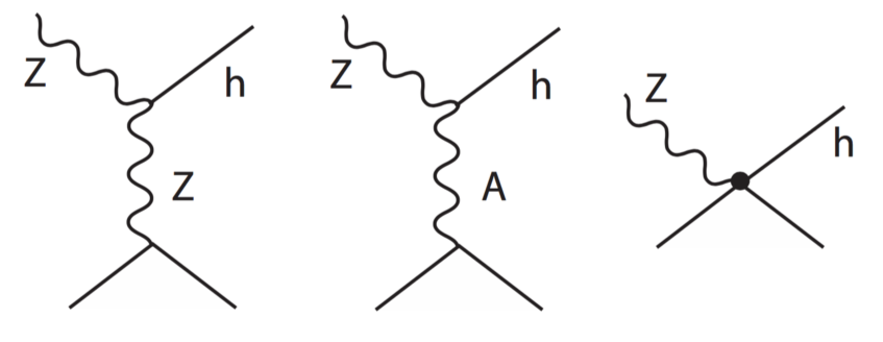
\includegraphics[width=0.80\hsize]{chapters/figures/Zhdiagrams.pdf}
\end{center}
\caption{Feynman diagrams contributing to the process $\ee\to Zh$ when 
contributing  dimension-6 operators are included. }
\label{fig:eeZhdiagrams}
\end{figure}
%%%%%%%%%%%%%%%%%%%%%%%%%%%%%%%%%%%%%%%%%%%%%%%%%%%%%%%%%%%%%%

%%%%%%%%%%%%%%%%
\begin{figure*}
\begin{center}
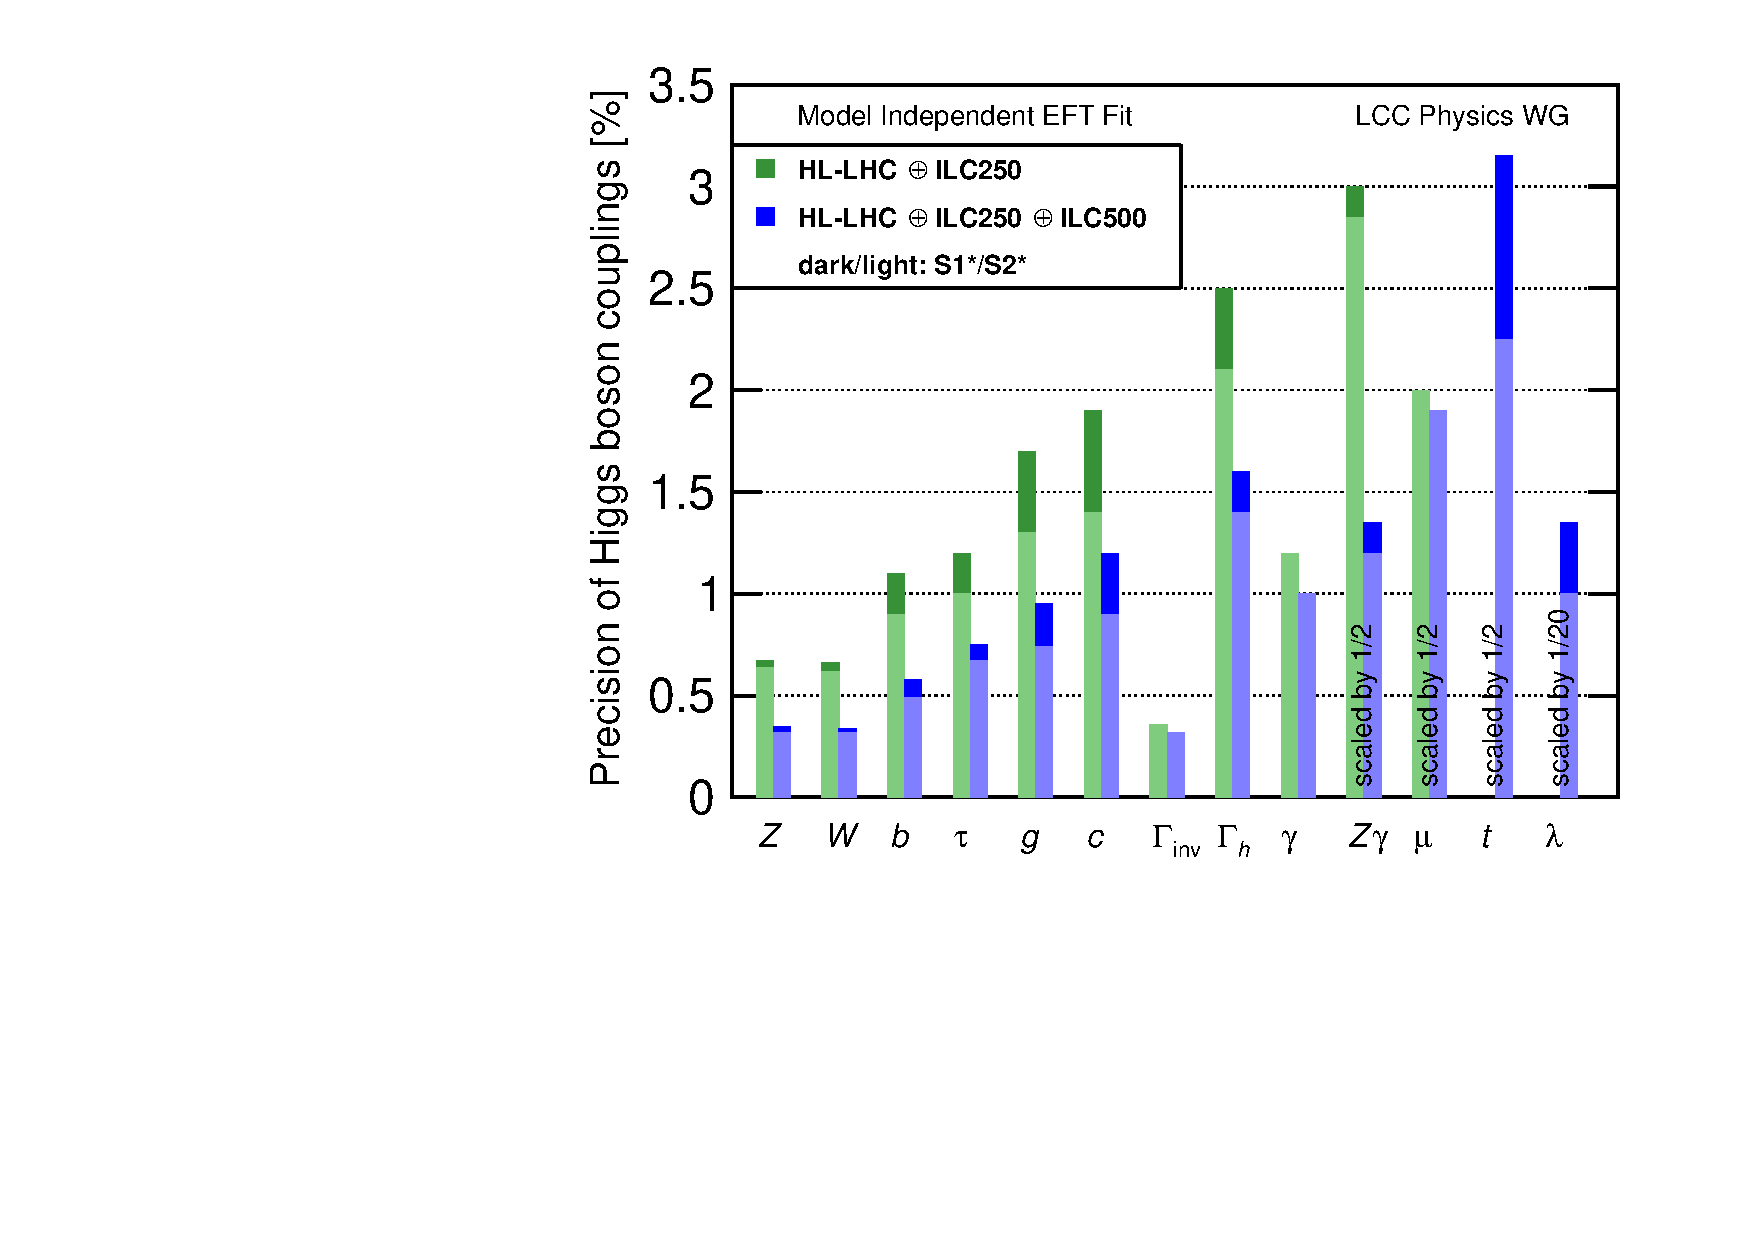
\includegraphics[width=0.7\hsize]{chapters/figures/DeltaHXX_SM_ILC_MI_S12s.pdf}
\caption{Projected Higgs boson coupling uncertainties for the ILC
  program at 250~GeV and an energy upgrade to 500~GeV, using the
  highly model-independent analysis presented in \cite{Fujii:2017vwa}. This
  analysis makes use of  data on $\ee\to W^+W^-$ in addition to Higgs
  boson observables and also incorporates projected LHC results, as described
  in the text.  These
values correspond to the  scenario S1* in Table~\ref{tab:ILCLHC}.}
\label{fig:ILCmodelindep}
\end{center}
\end{figure*}
%%%%%%%%%%%%%%%%%%%%%%%%%%%%%%%%%%%%%%%%%%%%%%%%%%%%%%%%%%%%%%
%
From this analysis, we derive the projected uncertainties on Higgs
couplings shown in Tab.~\ref{tab:ILCHiggs}.  We emphasize that the
analysis leading to these projections is completely model-independent,
in the sense that all models of new physics describable either by the
addition  of local operators to the SM EFT (for heavy new particles)
or by the addition of invisible and exotic Higgs decays (for light new
particles) are included.  These estimates give the
current state of our understanding of the ILC capabilities.  Given the
run plan and  detector designs described above, we have a high degree
of confidence that these estimated uncertainties will be achieved --
and, probably, surpassed -- in the realization of the ILC program.
The projections in the table are summarized in Fig.~\ref{fig:ILCmodelindep}.

%%%%%%%%%%%%%%%%%%%%%%%%%%%%%%%%%%%%%%%%%%%%5
\begin{table}[!htbp]
\begin{center}
\begin{tabular}{lcc}
   coupling     &   2~\iab\ at 250      &   + 4~\iab\ at 500   \\ \hline 
$HZZ$            &             0.67&            0.35                  \\ 
$HWW$            &         0.66               &   0.34    \\ 
 $Hbb$            &              1.1  &                0.58   \\ 
$H\tau\tau$    &          1.2  &                   0.74   \\ 
$Hgg$ &  1.7  &       0.95          \\ 
$Hcc$         &   1.9  &  1.2  \\ 
$H\gamma\gamma$ &  1.2 &   1.0  \\ 
$H\mu\mu$ &  5.6  &  5.1  \\ 
$Htt$  &   -     &      6.3   \\ 
\hline 
$HHH$  &  -    &   27   \\ \hline 
$\Gamma_{tot}$ & 2.5  & 1.6  \\  
$\Gamma_{inv}$ &   0.32  & 0.29 \\  \hline
\end{tabular}
\end{center}
\caption{ \label{tab:ILCHiggs}    Projected uncertainties in the Higgs
  boson couplings for the ILC at 250~GeV and 500~GeV, with
  precision LHC input, assuming the
  integrated luminosities in the H20 program.   All values
  are given in percent (\%). The ILC at 250~GeV only does 
not have direct sensitivity to the $Htt$ and $Hhh$ couplings; thus no  model-independent  values are given in these lines. The
  bottom lines give, for reference, the projected uncertainties in the
  Higgs boson total width and the 95\% confidence limits on the Higgs
  boson invisible width.
   The analysis, which applies Effective Field Theory as described in
   the text,  is highly model-independent}
\end{table}





\subsection{Systematic uncertainties and the importance of beam polarization}
\label{subsec:polarisation}


  For the studies of the Higgs boson in which we wish to claim that precisely measured deviations from the SM can give a discovery of new physics, we must be certain that systematic errors are both small and well-constrained.  In this section, we will discuss 
the sources of systematic error that we consider in our Higgs coupling analysis.

We will also discuss the capability that the ILC gives to control systematic uncertainties using the availability of polarized beams. In precision measurement, it is useful, whereever possible, to  measure effects correlated to sources of systematic uncertainty.  For this, it is crucial to always have one more degree of freedom that (statistically) absolutely required.  In the ILC program, electron and positron polarisation
provide tools to validate estimates of systematic errors, and to reduce these 
sources of uncertainty.  In Sec.~\ref{subsec:beampol}, when we reviewed in general terms the importance of the
 use of beam polarisation to meet the physics goals of the ILC, we did not emphasize this 
aspect of the physics implication of polarisation.  But it is clear that, for each measurement that can be done at an unpolarized collider, a collider with control of the polarization for each beam can provide four independent data sets.  We will explain in this section how this tool 
can be used not only to estimate but also to reduce systematic errors.


\subsubsection{Systematic uncertainties considered in the Higgs coupling fit}
\label{subsubsec:sysuncert}
The evaluation of systematic uncertainties for experiments which have not yet been built is a difficult task and will to some extent always remain guess-work until real data have been taken. To some extent, we can rely on the experience from previous $e^+e^-$ experiments, especially at LEP, where many uncertainties could be controlled to a typical level of 1\%.
The ILC detector designs, which aim for higher precision, make use of this experience,
as explained in Sec.~\ref{sec:detectors}.  Assuming this basic level of performance, detailed studies of systematic uncertainties at the ILC have concentrated on cases where the statistical uncertainties are expected to be significantly below 1\%, and on searches in channels with large irreducible backgrounds. An example for the first case is a global analysis of total rates and differential distributions of various 2-fermion and 4-fermion SM processes, extracting simultaneously the total unpolarised cross sections, the relevant left-right asymmetries, the beam polariations and the charged triple gauge couplings, see Sec.~\ref{subsec:ew_WWana} and Ref.~\cite{bib:PhDRobert}. An illustrative example for the second category, though not directly connected to Higgs physics, is the WIMP search in the mono-photon channel, see Sec.~\ref{sec:searches} and Ref.~\cite{Habermehl:417605}. 

Studies of this type lead us to the following estimates of the dominant systematic uncertainties (previewed already at the end of Sec.~\ref{subsec:higgs_ana}).  These sources of systematic uncertainty are also applied to the measurements of triple gauge boson couplings described 
in Sec.~\ref{subsec:ew_WWana}.
\begin{itemize}
\item The luminosity at the ILC will be measured from low-angle Bhabha scattering with the help of a dedicated forward calorimeters, the LumiCals (see Sec.~\ref{subsub:det:forward} and Ref.~\cite{Abramowicz:2010bg}). This measurement is extremely sensitive to the exact alignment of the LumiCals on the two sides of the detector, as well as to beam backgrounds and has been studied in detailed simulations both for the ILC and for CLIC~\cite{Bozovic-Jelisavcic:2014aza, Lukic:2013fw}. Based on these studies, the resulting systematic uncertainty on all Higgs cross section and cross-section-times-braching-ratio measurements is assumed to be 0.1\%
\item Another 0.1\% is assumed for the net systematic effect of the finite knowledge of luminosity-weighted long-term average values of the beam polarisations at the $e^+e^-$ interaction point.    Compton polarimeters in the Beam Delivery System will provide 
time-stable measurements of the beam polarizations at their locations at the level of 0.25\%~\cite{Vormwald:2015hla, List:2015lsa}.  To obtain the polarizations relevant for 
the experiments, one must also consider also the effects of spin transport, misalignment of beam line magnets as well as depolarisation during the beam-beam interaction~\cite{Beckmann:2014mka}. The absolute scale of the luminosity-weighted average polarisation at the IP is finally calibrated from collision data, \eg, from a global fit to SM processes with strong polarisation dependence~\cite{bib:PhDRobert}. 
\item Theoretical uncertainties are also assumed to have reched at the level of 0.1\% by the time of ILC operation.   This requires the computation of all relevant processes to 2 loops in the electroweak interactions, a task feasible within the current state of the art~\cite{Blondel:2019qlh}.  Another question is the availability of high-precision values for the most important input parameters---$m_b$, $m_c$, $\alpha_s$, and $m_h$.  We expect to obtain the first threee  of these to sufficient accuracy from lattice QCD~\cite{Lepage:2014fla}.
For $m_h$, the  ILC recoil measurement described in Sec.~\ref{sec:higgs:sigmazh} will provide 
the high precision needed.
\item For flavor tagging, systematic errors of 1\% have already been reached at LEP.. With the advances in detector technology and the larger integrated luminosity, we assume that for each data set at the ILC this can be reduced  and also improved as  a function of integrated luminosity by probe-and-tag measurements.   We expect an uncertainty of 
$0.3\% \sqrt{0.250/L}$, where $L$ is the integrated luminosity in iab.  This is an error of 0.1\% for the ILC250.
% , improving  These 0.3\% are considered as net effect of all experimental uncertainties in the absence of beam polarisation.

% In the presence of both beam polarisations, the net effect of systematic uncertainties has been shown to be smaller by factors between 2 and 10 due to the correlations between data sets with different beam polarisations as discussed in Sec.~\ref{subsubsec:pol:systematics}. Since the Higgs coupling fit does not yet comprise such a detailed treatment of systematic uncertainties and their correlations as the above mentioned global fit to 2-fermion and 4-fermion processes, we assume that, in presence of polarised beams, the net effect of the experimental uncertainties reduces to 0.1\%.


\end{itemize}



\subsubsection{Control of systematic uncertainties using beam polarisation} 
\label{subsubsec:pol:systematics}

In the remainder of this section we will highlight the impact of the beam polarisation on the control of systematic uncertainties using these two studies as examples.   We have already pointed out that beam polarisation provides subsets of the data that can be used as cross-checks of systematic errors on 
efficiencies for signal identification and background suppression.  However, the studies
in Refs.~ \cite{Habermehl:417605} and \cite{bib:PhDRobert} and go beyond this to illustrate the use of beam polarisation to actually reduce systematic errors beyond what is possible at 
an unpolarised collider.   Both of these studies were carried out for measurements at the 
500~GeV ILC, but the same principles apply to the 250~GeV data.

Several principles combine to produce this  result.   The first is that different polarization
settings produce event samples with different mixtures of signal and background 
processes.   The differences in these  mixtures arise from order-1 polarization asymmetries that vary from 
process to process, to first approximation, in the manner predicted by the SM.   In the SM, for example, lepton pair production has a small polarization asymmetry while the   polarization asymmetry for $b\bar b $ production is large and that for $W$ pair production is almost maximal.   For certain modes, for example, lepton pair production and di-jet production, the detection  efficiency is naturally very high and therefore has a small uncertainty, while for other processes, for example, $b\bar b$ production, this efficiency is smaller and also more complicated to estimate.  If we introduce nuisance factors for the more uncertain efficiencies
and determine these from data, the correlation of the relative compositions with polarization
allows us to determine these parameters in terms of the efficiencies that are better known. 

The second principle is that systematic uncertainties that are correlated with polarization can be cancelled locally in the data set using fast reversal of the beam helicities.  This principle 
was essential to the excellent measurement of $\sin^2\theta_w$ by the SLD experiment 
from a very small data sets; almost all systematic errors were cancelled by flipping the $e^-$ beam  polarization in a pseudo-random fashion~\cite{Abe:1996nj}.   The principle of rapid helicity reversal is built into the ILC design, which gives the capability to flip the sign of 
polarisation for each of the two beams independently on a train-by-train basis (see Sec.~\ref{par:beampol}.  This helicity reversal is fast compared to typical time-scales of changes in the configuration, calibration, and alignment of the detector and the accelerator.
It implies that data sets with the same beam energy but different beam helicities can be considered as being collected  essentially concurrently.  

%%%%%%%%%%%%%%%%%%%%%%%%%%%%%%%%%%%%
\begin{figure}
\centering
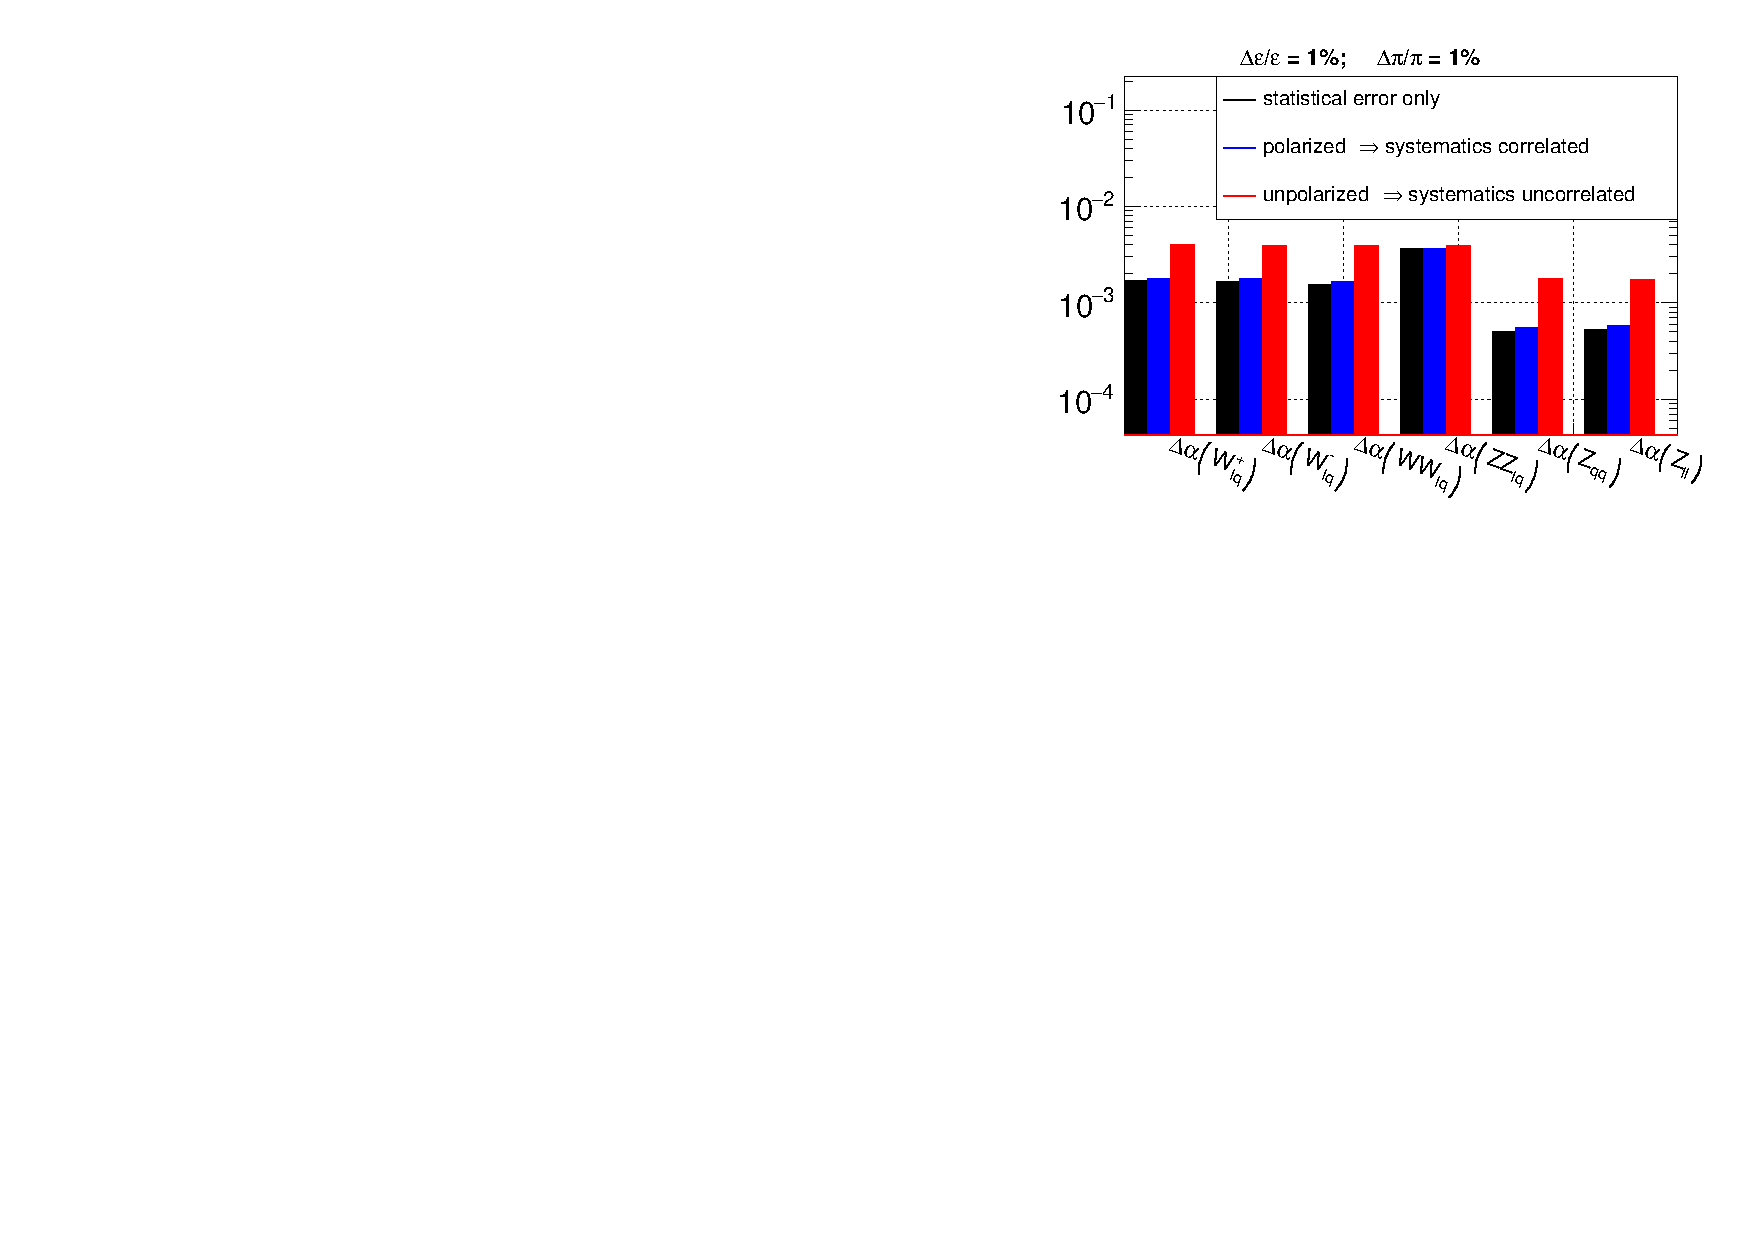
\includegraphics[width=0.95\linewidth]{./chapters/figures/ElectroWeakSysDependency_alpha_short.pdf}
		
\caption{Uncertainties on the unpolarised cross sections of various 2-fermion and 4-fermion processes as obtained from the global fit introduced in the text~\cite{bib:PhDRobert}, assuming a systematic uncertainty of 1\% on the selection efficiencies and purities, each. In the case of polarised beams, it is estimated that only 10\% of the uncertainty is uncorrelated between data sets.  Applying that estimate to the analysis of data sets taken ``quasi-concurrently", the impact of the systematic uncertainties is minimal.  Without the redundancies provided by data sets with correlated systematic uncertainties, the total uncertainties increase by a factor 2 for $WW$ and single-$W$ processes and a factor of 5 for 2-fermion processes.}
\label{fig:alpha_error_corr_uncorr}
\end{figure}
%%%%%%%%%%%%%%%%%%%%%%%%%%%%%%%%%%%%%%


The improvement in the measurement of the absolute normalization of cross sections can be very significant.  The study of Ref.~\cite{bib:PhDRobert} considered the full set of 2-fermion production processes and 4-fermion production processes (including $\ee\to WW / ZZ \to 4$~fermions and well as single-$W$ production) at 250~GeV.   Each channel was assigned a 1\% systematic uncertainty in its selection efficiency and signal purity. Based on the correlations of experimental effects between ``quasi-concurrently'' taken data sets, discussed in section~\ref{subsubsec:pol:systematics}, it was estimated that only 10\% of this uncertainty is uncorrelated between data sets with different the beam polarisation configurations. Thus, a global fit using all four
polarization settings allows one to determine the relative efficiencies and remove most of the systematic uncertainty.  The result for the final normalization uncertainties are shown in 
Fig.~\ref{fig:alpha_error_corr_uncorr}.  For each of several 2- and 4-fermion channels, the black bars show the statistical uncertainties, the red bars show the full uncertainties for unpolarised data, and the blue bars show the uncertainties for polarised data samples.   The final uncertainties are larger in unpolarized case by a factor of 2 for $WW$ and single-$W$ processes and by a factor of 5 for lepton pair production.

%%%%%%%%%%%%%%%%%%%%%%%%%%%%%%%%%%%%%%%%%%%%%%
\begin{figure}
\centering
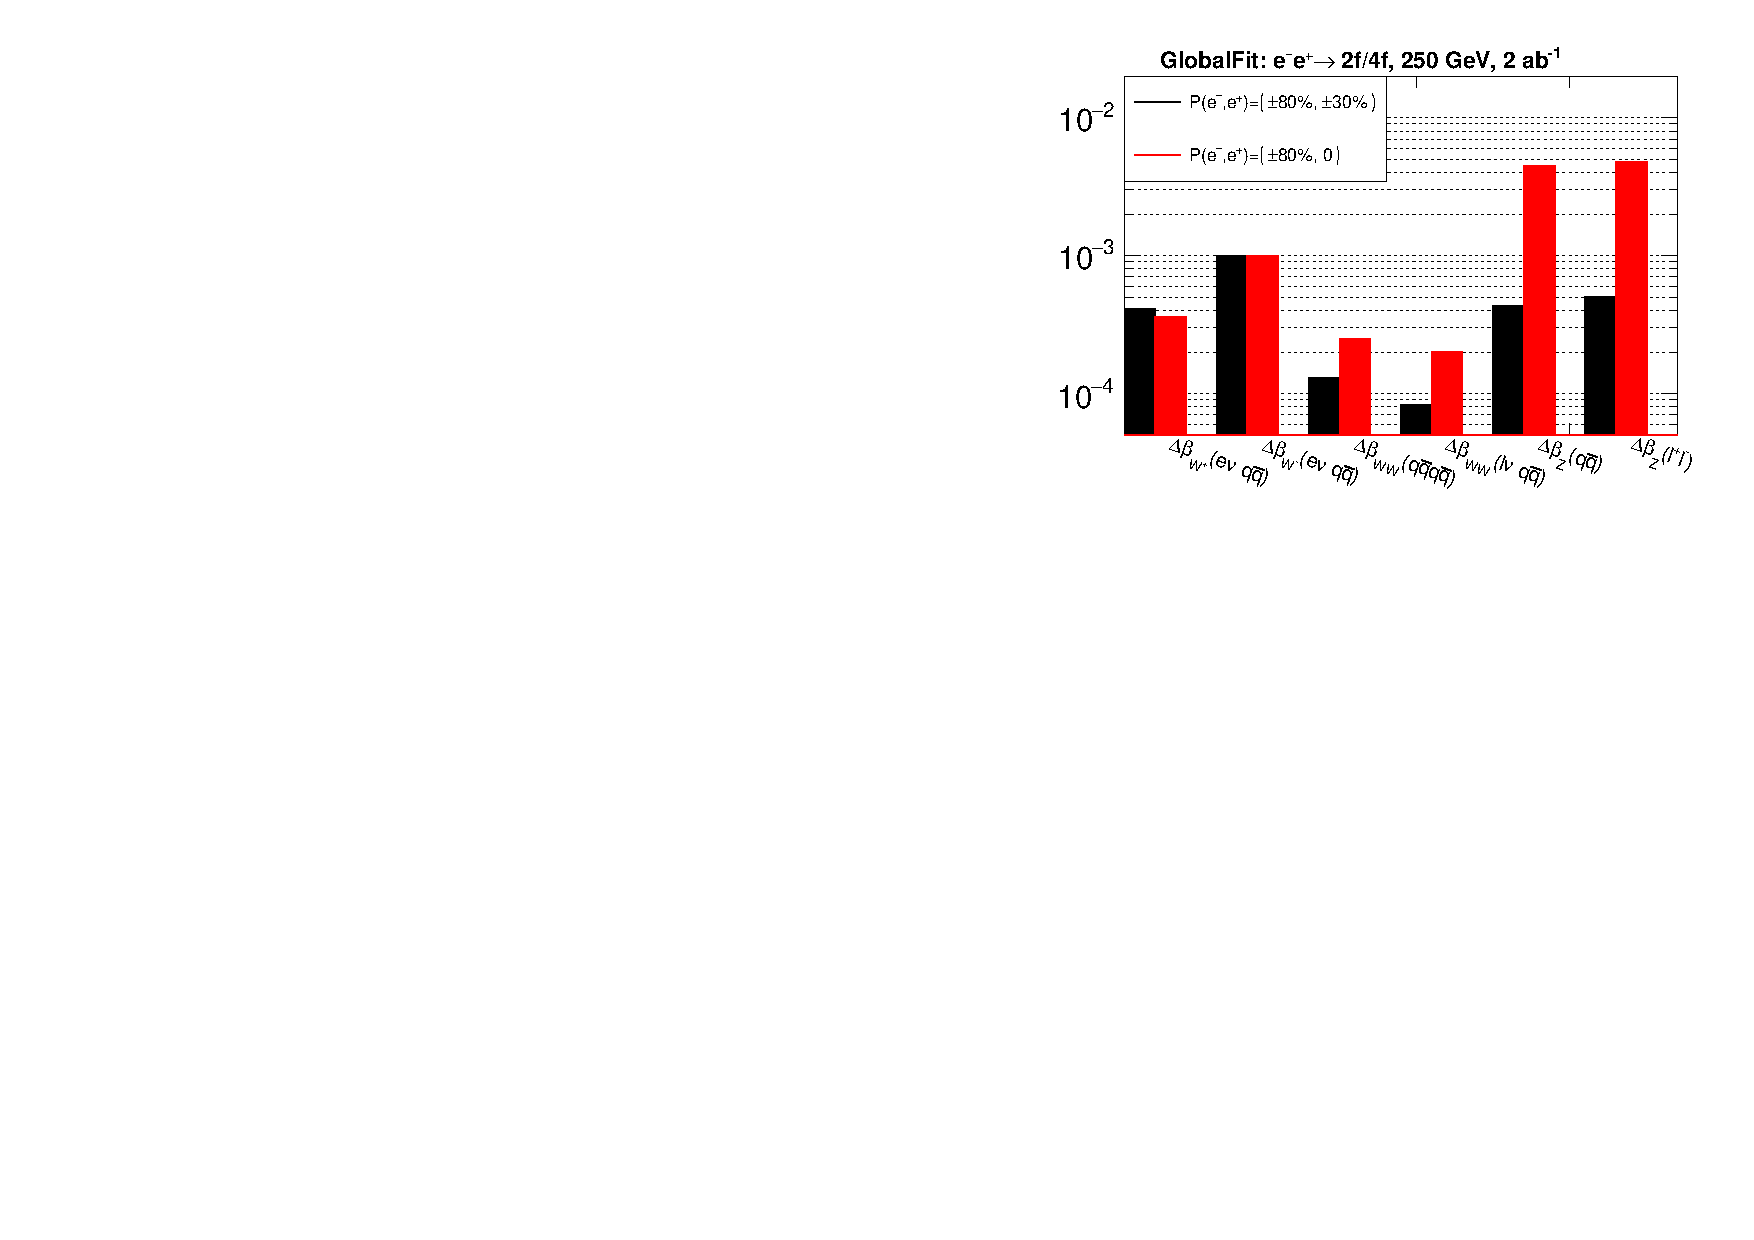
\includegraphics[width=0.95\linewidth]{./chapters/figures/beta_precision_upolarized.pdf}
		
\caption{Uncertainties $\Delta \beta$ on \ALR\ of various 2-fermion and 4-fermion processes as obtained from the global fit introduced in the text~\cite{bib:PhDRobert} with both beams polarised (with the standard 45\%/45\%/5\%/5\% sharing between the four helicity configurations) and in the absence of positron polarisation (with a 50\%/50\% sharing between the two remaining helicity configurations). In the absence of positron polarisation, the  uncertainties on \ALR\ increase by a factor 2 for $WW$ and by about a factor of 10 for 2-fermion processes. Alone the single-$W$ processes remain unaffected.}
\label{fig:beta_error_noposipol}
\end{figure}
%%%%%%%%%%%%%%%%%%%%%%%%%%%%%%%%%%%%%%%%%%%%%%


The same principles can be applied to the measurement of polarisation asymmetries $A_{LR}$, which, as we have seen, play a large role in the ILC program.   Though many systematic 
errors automatically cancel in $A_{LR}$, there are new sources of systematic uncertainty, for example, the possibility of a correlation between the helicity orientation and the luminosity delivered per bunch train.   This is effectively controlled if both the electron and positron 
bunches can be polarised.  Roughly, the polarization asymmetry in $W$ pair production is almost maximal, and the small uncertainty in this quantity can be transferred to the value of $A_{LR}$ for other processes. The point is illustrated in Fig.~\ref{fig:beta_error_noposipol}, again from Ref.~\cite{bib:PhDRobert}, which shows a comparison of the final uncertainty on 
$A_{LR}$ in a global fit between a collider with $e^-$ and $e^+$ polarization (black bars) and a collider with only $e^-$ polarization (red bars). The improvement is a factor of 10 for 
fermion pair production.  (In this illustrative study, the systematic errors from detector efficiency and theory are set equal to zero.) 

%%%%%%%%%%%%%%%%%%%%%%%%%%%%%%
\begin{figure}
\centering
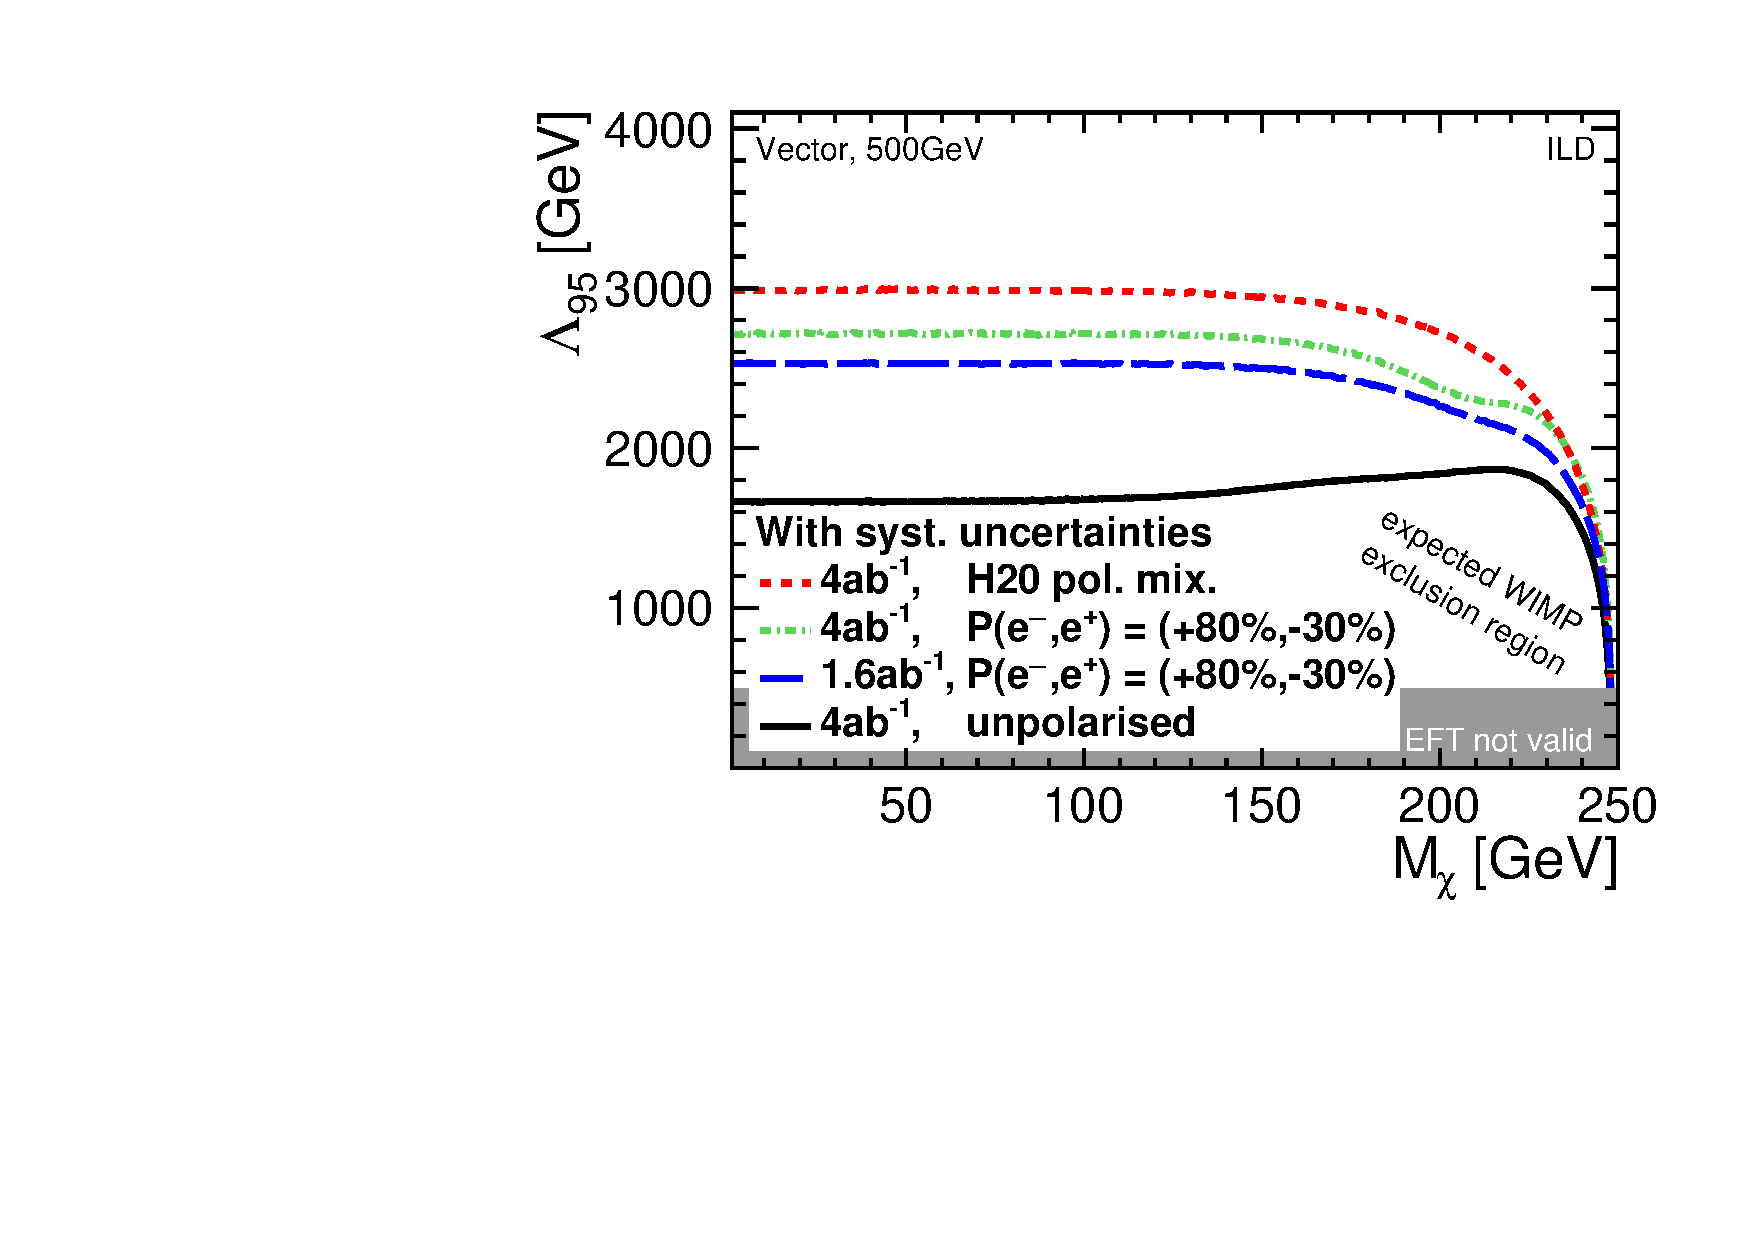
\includegraphics[width=0.95\linewidth]{./chapters/figures/vector_withSystematics.pdf}
		
\caption{Comparison of the reach of the search for WIMP production in the mono-photon channel for different assumptions on luminosity and polarization, {\em including} systematic uncertainties (see Sec.~\ref{sec:searches} for a description of the analysis)~\cite{Habermehl:417605}. }
\label{fig:polWIMPsys}
\end{figure}
%%%%%%%%%%%%%%%%%%%%%%%%%%%%%%%%%%%


Similar large effects from polarisation are seen in cases in which the signal is detected in 
the shape of  a  distribution.    An illustration here is given by a study of the search for 
dark matter particles $\chi$ using the mono-photon signature~\cite{Habermehl:417605}, already discussed in Sec.~\ref{subsec:beampol}.   In our earlier discussion, we pointed out that the signal from 
$\ee\to \gamma \chi\chi$ sits on top of a large irreducible background from 
$\ee\to \gamma \nu\bar \nu $.  The study includes a careful evaluation of the systematic uncertainties, including those on selection efficiencies, luminosity, beam energy (spectrum) and polarization as well as on the theoretical modelling of the background. 
The limit calculation uses fractional event counting based on the observed energy spectrum of the selected photon candidates and considers normalisation and shape-dependent uncertainties as well as the correlations between these. If the mass of the $\chi$ is relatively high, only low-energy photons can appear in the signal process.  Then the high-energy part of the photon spectrum can be used to determine nuisance parameters assigned to the 
polarization and efficiencies.  The results for the lower limit on the mediator scale, including 
systematic errors, are shown in Fig.~\ref{fig:polWIMPsys}. This figure should be compared to 
Fig.~\ref{fig:polWIMPstat}, in which systematic errors are set to zero.   Note that, in this case, the strongest limits are set using a mixture of beam polarizations (the dashed red curve in both cases) since this allows the systematic errors from beam polarisation to be better 
controlled.









\subsection{Comparison of run scenarios for linear and circular $\ee$ collliders}
\label{subsec:lincirc}



In this section, we will present a comparison of the capabilities of
the ILC for precision Higgs measurement with those of other proposed
linear and circular colliders, including CLIC, CEPC, and FCC-ee.  We
will present two sets of comparisons, organized in the 
following way:

To begin, each collider proposal has presented its own set of
projections in its documentation for the European strategy study.   We
have copied the relevant numbers for projected Higgs boson coupling
uncertainties into Tab.~\ref{tab:askthem}. 
 These estimates are made using the more model-dependent
 kappa fit.   (The small values of the $ZZ$ coupling uncertainty relative to the $WW$ coupling uncertainty reflects the model-dependence discussed above.)


%%%%%%%%%%%%%%%%%%%%%%%%%%%%%%%%%%%%%%%%%%%%5
\begin{table*}[!htbp]
\begin{center}
\begin{tabular}{l|cc|c|c|ccc}
    &  ILC250      &   ILC500   & CEPC &  FCC-ee &
   CLIC350 & 
   CLIC1.4 & CLIC3 \\ 
coupling &   EFT fit & EFT fit & $\kappa$ fit &  $\kappa$ fit &
                                                                $\kappa$
                                                                fit &
                                                                      $\kappa$
                                                                      fit
   $\kappa$ fit & \\ \hline 
$HZZ$            &             0.67&   0.35    &   0.25   & 0.17     &  0.6     &     0.6    &   0.6     \\ 
$HWW$            &         0.66  &   0.34   &   1.4   &   0.43   &   1.0    &   0.6  &  0.6 \\ 
 $Hbb$            &              1.1  &  0.58   &  1.3    &    0.61  &   2.1    &  0.7  &  0.7 \\ 
$H\tau\tau$    &          1.2  &   0.74   &   1.5   &  0.74    &   3.1    &  1.4  &  1.0 \\ 
$Hgg$ &                      1.7  & 0.95       &  1.5    &  1.01    &   2.6    &   1.4   &  1.0  \\ 
$Hcc$                       &   1.9  &  1.2   &   2.2   &   1.21   &    4.4   &  1.9  &  1.4 \\ 
$H\gamma\gamma$ &  1.2 &   1.0     &  1.6    &   1.3   &    -   &  4.8  &  2.3 \\ 
$H\mu\mu$                &  5.6  &  5.1     &  5.0    &  3.8    &    -
& 12.1 &  5.7 \\ 
$Htt$  &                       -     &      6.3     &  -    &  -    &
-    & 3.0  &  3.0  \\ 
$HHH$                         &  -    &   27     &   -   &   -   &   -
& 35 &  9 \\ \hline 
$\Gamma_{tot}$             & 2.5  & 1.6    &   2.8    &  1.3     &
4.7    & 2.6  & 2.5 \\  
$\Gamma_{inv}$          &   0.32  & 0.29    &  < 0.3    &   -   &   -
& -  & - \\  \hline
\end{tabular}
\end{center}
\caption{ \label{tab:askthem}    Projected uncertainties in the Higgs
  boson couplings quoted in the CDRs presented to the European
  Strategy Study.  The methodology of the fit is indicated. 
 For the ILC, the  values are taken from
  Tab.~\ref{ILCHiggs}.    For the CEPC, the values are taken from
  Ref.~\cite{CEPCStudyGroup:2018ghi}, Tab.~11.4.  For the FCC-ee, the values are taken
  from Ref.~\cite{Benedikt:2018qee}, Tab.~1.2. As discussed later,
  the capability for $\Gamma_{inv}$  is similar to that for CEPC. 
 For CLIC, the values are taken from 
Ref.~\cite{Charles:2018vfv}, Tab.~2, with $HHH$ values from
Ref.~\cite{Roloff:2019crr}.
  All values
  are given in percent (\%). The
  bottom lines give, for reference, the projected uncertainties in the
  Higgs boson total width and the 95\% confidence limits on the Higgs
  boson invisible width.  For  ILC, CEPC, and FCC-ee, the 
 values given for the $\gamma\gamma$ and $\mu\mu$ modes are those
 combined with expected
LHC results.}
\end{table*}



It is interesting to ask how the proposals would compare if a common
fitting technique is used. In almost all cases, the measurement errors
are dominated by statistics and the efficiencies used in the analyses
are similar.  A simple way to make the comparison is  to use
the results of our ILC analyses to estimate efficiencies and
statistical errors for all of the colliders.  That is, we can  assume
the luminosity samples in the collider proposals, assume the same
measurement errors per unit of luminosity that we assumed in
generating Tab.~\ref{tab:ILCHiggs},  take account of differences in
the cross sections resulting from the use (or not) of polarized beams,
and rerun our fitting  program for those conditions.   This is the
method used to generate 
Tab.~3 of Ref.~\cite{Barklow:2017suo}.  To model CEPC, we assume
 a sample of  5~\iab\ at 250~GeV without polarization; for 
FCC-ee, we use a sample of 5-\iab at 250~GeV plus 1.5~\iab\ at 350~GeV,
without polarization.  The run plan for CLIC includes only 1~\iab\ at
380~GeV before the energy upgrade to 1~TeV.  Since we are
unconfortable using the EFT formalism
 with dimension-6 operators only at 1~TeV and above, we represent CLIC by a sample of
2~\iab, similar to ILC, with 80\% $e^-$ polarization only, at 350~GeV.  
The results are presented in Tab.~\ref{tab:oursimple} and visualised in Fig.~\ref{fig:oursimple}.  


%%%%%%%%%%%%%%%%%%%%%%%%%%%%%%%%%%%%%%%%%%%%5
\begin{table*}[!htbp]
\begin{center}
\begin{tabular}{l|cc|c|c|c}
 &  2/ab-250 & +4/ab-500 &  5/ab-250 &  + 1.5/ab-350 &  2/ab-350 \\
coupling &  pol.  &   pol.  &   unpol.  &  unpol &  $e^-$  pol. 
  \\  \hline 
$HZZ$            &             0.67&   0.35    &   0.75   & 0.40     &  0.57            \\ 
$HWW$            &         0.66  &   0.34   &   0.75   &   0.40   &   0.57    \\ 
 $Hbb$            &              1.1  &  0.58   &  0.94    &    0.65  &   1.1   \\ 
$H\tau\tau$    &          1.2  &   0.75   &   1.0   &  0.74    &   1.3     \\ 
$Hgg$ &                      1.7  & 0.95       &  1.3    &  0.98    &   1.6    \\ 
$Hcc$                       &   1.9  &  1.2   &   1.4   &   1.1   &    2.3  \\ 
$H\gamma\gamma$ &  1.2 &   1.0     &  1.2    &   1.0   &    1.1    \\ 
$H\gamma Z$ &  6.0 &   2.6     &  9.2    &   6.9   &    4.5    \\
$H\mu\mu$                &  4.0  &  3.8     &  3.8    &  3.7    &    4.0
 \\ 
$Htt$  &                       -     &      6.3     &  -    &  -    &
-     \\ 
$HHH$                         &  -    &   27     &   -   &   -   &   -
 \\ \hline 
$\Gamma_{tot}$             & 2.5  & 1.6    &   2.0    &  1.5     &
2.5    \\  
$\Gamma_{inv}$          &   0.36  & 0.32    &  0.34    &  0.30   &   0.58
\\  \hline
\end{tabular}
\end{center}
\caption{ \label{tab:oursimple}    Projected uncertainties in the Higgs
  boson couplings computed using the EFT method, with  ILC uncertainties per unit of luminosity and assuming a run with the quoted integrated luminosity
  and energy.   The first two columns are the ILC values from 
  Tab.~\ref{ILCHiggs}.   In the last column, we assume 80\% electron polarization and zero positron polarization.  }
\end{table*}
%%%%%%%%%%%%%%%%
\begin{figure*}
\begin{center}
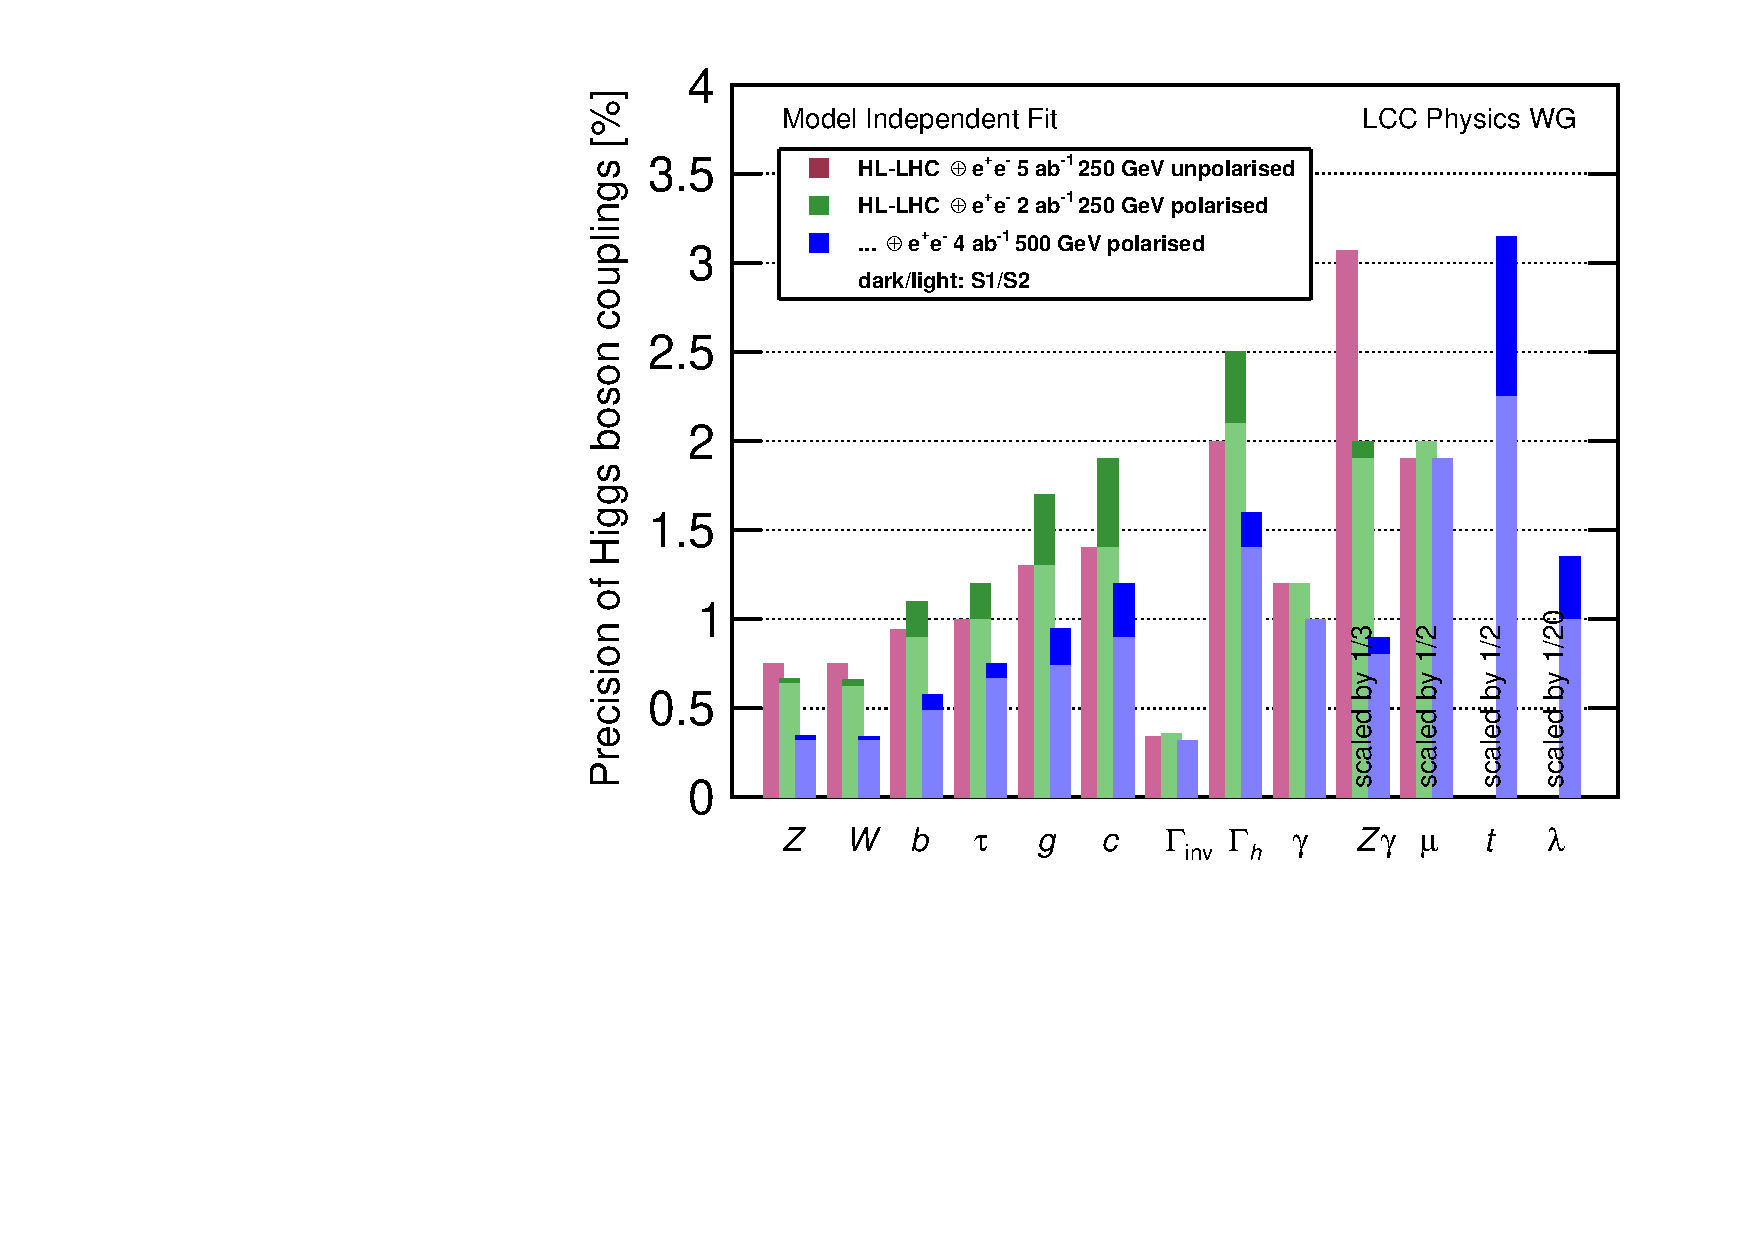
\includegraphics[width=0.7\hsize]{chapters/figures/DeltaHXX_SM_ILC_LEP_MI.pdf}
\caption{Projected Higgs boson coupling uncertainties for selected scenarios from Table~\ref{tab:oursimple}.
In particular it shows that at $\sqrt{s}=250$\,GeV, 2\,\iab  with polarised beams yield comparable results to a much larger data set of 5,\iab with unpolarised beams.}
\label{fig:oursimple}
\end{center}
\end{figure*}
%%%%%%%%%%%%%%%%%%%%%%%%%%%%%%%%%%%%%%%%%%%%%%%%%%%%%%%%%%%%%%


Though not all differences among the various proposals are included in
this table, it does usefully show how increased luminosity trades off
against beam polarization.   We see that beam polarization is a very
powerful tool, essentially compensating the advantage of larger event
samples claimed by the circular machines.   The comparison of 2~\iab\
data samples at 250 and 350~GeV is also interesting, since the two
energy settings bring different advantages to the Higgs physics study.


Finally, it is interesting to ask how improved precision electroweak
measurements affect these numbers. For ILC, we include the improved 
measurements of $Z$ pole parameters  from the Giga-Z program,
described
in Sec.~\ref{sec:gigaz}.  For the circular colliders, 
we include the improvement in
precision electroweak measurements expected from the program of $Z$
pole described in the FCC-ee CDR~\cite{Benedikt:2018qee}. The results are presented in 
Tab.~\ref{tab:ournotsosimple}and visualised in Fig.~\ref{fig:outnotsosimple}. 

%%%%%%%%%%%%%%%%%%%%%%%%%%%%%%%%%%%%%%%%%%%%5
\begin{table*}[!htbp]
\begin{center}
\begin{tabular}{l|cc|c|c}
 &  2/ab-250 & +4/ab-500 &  5/ab-250 &  + 1.5/ab-350\\
coupling &  pol.  &   pol.  &   unpol.  &  unpol  
  \\  \hline 
$HZZ$            &             0.52&   0.34    &   0.51   & 0.36            \\ 
$HWW$            &         0.52  &   0.34   &   0.52   &   0.37    \\ 
 $Hbb$            &     1.0  &  0.58   &  0.78    &    0.63       \\ 
$H\tau\tau$    &          1.1  &   0.74   &   0.86   &  0.72      \\ 
$Hgg$ &                      1.6  & 0.95       &  1.2    &  0.97     \\ 
$Hcc$                       &   1.8  &  1.2   &   1.3   &   1.1    \\ 
$H\gamma\gamma$ &  1.1 &   1.0     &  1.1    &   1.0   \\ 
$H\gamma Z$ &  3.9 &   2.3     &  9.0    &   6.8     \\
$H\mu\mu$                &  4.0  &  3.8     &  3.8    &  3.7   
 \\ 
$Htt$  &                       -     &      6.3     &  -    &  -     \\ 
$HHH$                         &  -    &   27     &   -   &   -  \\ \hline 
$\Gamma_{tot}$             & 2.3  & 1.6    &   1.7    &  1.4       \\  
$\Gamma_{inv}$          &   0.36  & 0.32    &  0.34    &   0.30  \\  \hline
\end{tabular}
\end{center}
\caption{ \label{tab:ournotsosimple}    Projected uncertainties in the Higgs
  boson couplings computed using the same methodology as
 in Tab.~\ref{tab:oursimple} but including projected improvements in
 precision electroweak measurements.  At this moment (as I understand it
 - MEP ) the uncertainties on precision electroweak results described
 in the 
 FCC-ee CDR~\cite{Benedikt:2018qee} are used in all columns.   It
 would be interesting to add 2 columns with ILC + Gigaz.}
\end{table*}

%%%%%%%%%%%%%%%%
\begin{figure*}
\begin{center}
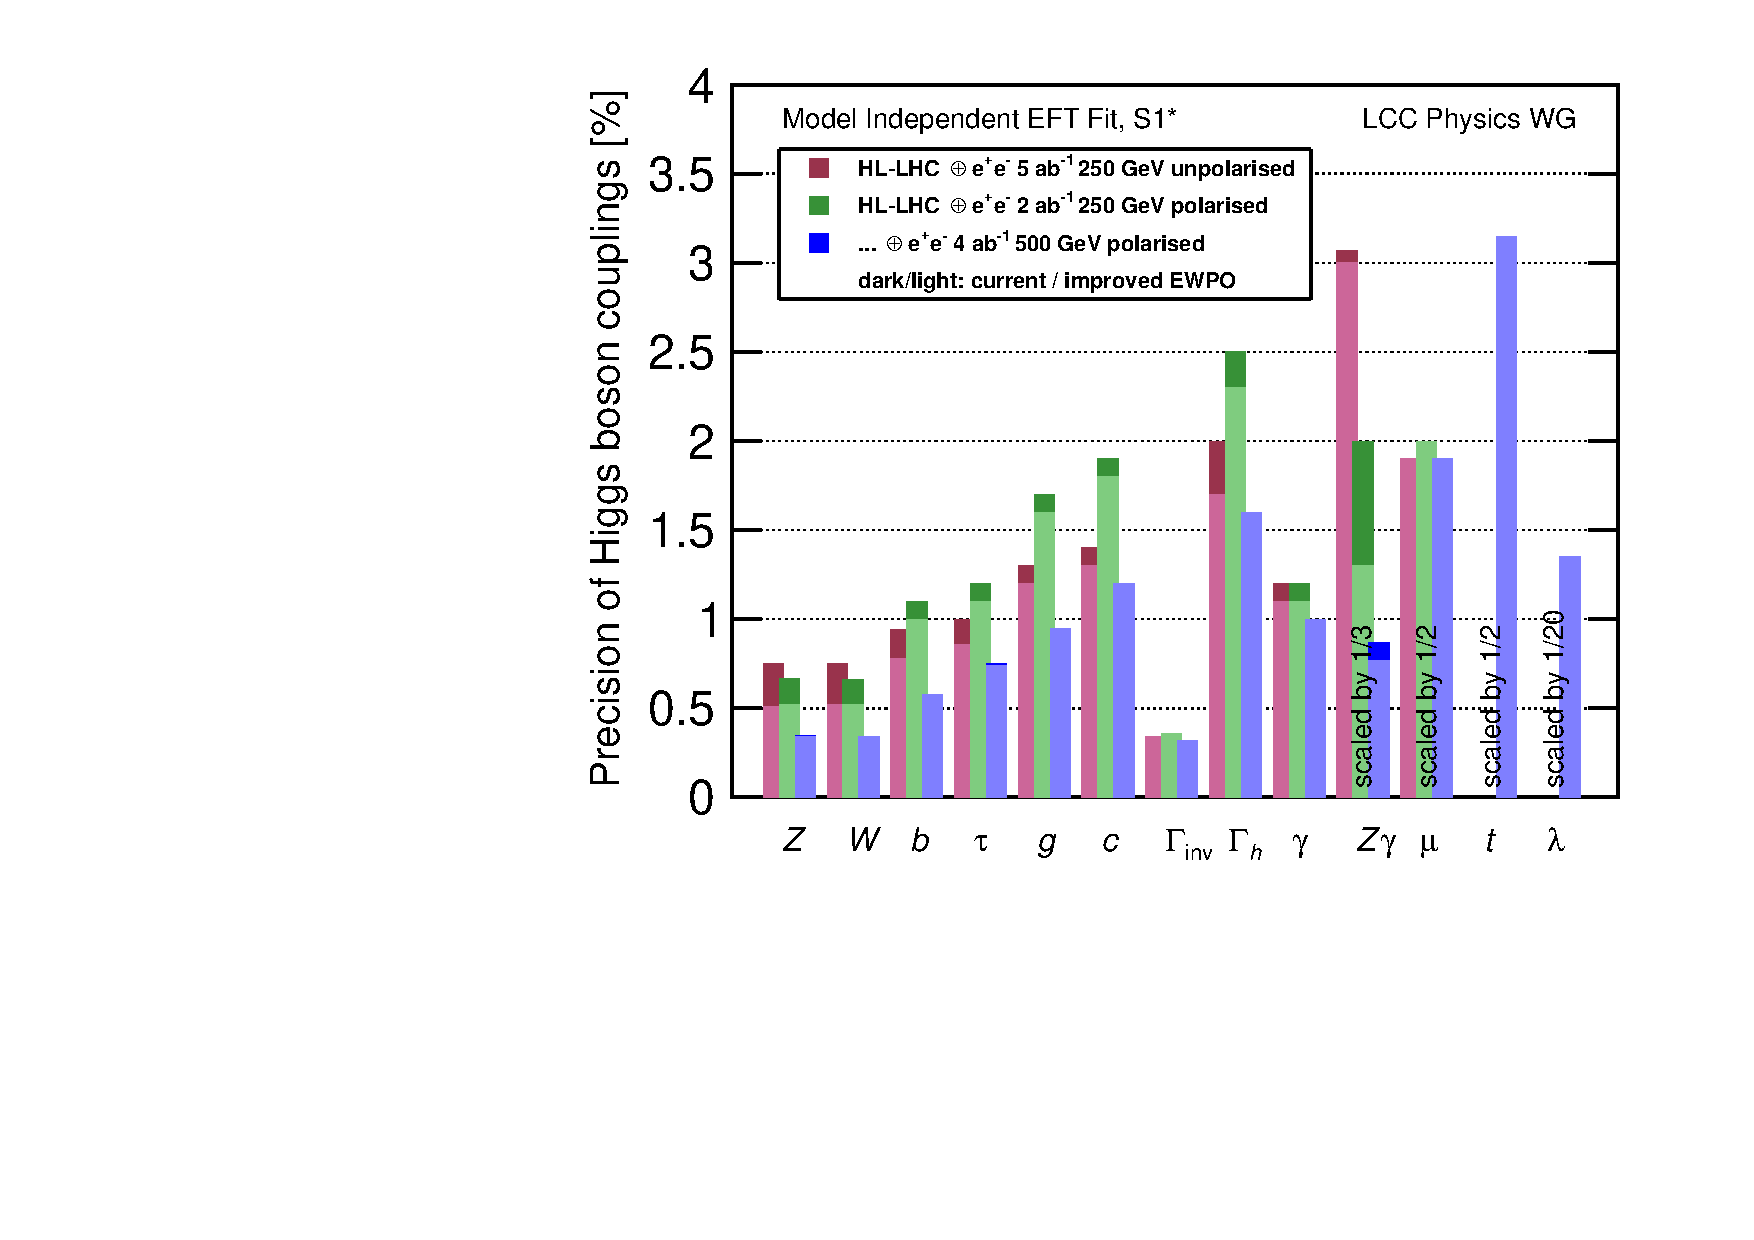
\includegraphics[width=0.7\hsize]{chapters/figures/DeltaHXX_SM_ILC_EWPO_MI.pdf}
\caption{Projected Higgs boson coupling uncertainties for selected scenarios from Table~\ref{tab:ournotsosimple}, illustrating the impact of improved electroweak precision observables in the cases of $\sqrt{s}=250$\,GeV -- 2\,\iab\ polarised and 5\,\iab\ unpolarised -- and for $\sqrt{s}=500$\,GeV.}
\label{fig:ournotsosimple}
\end{center}
\end{figure*}
%%%%%%%%%%%%%%%%%%%%%%%%%%%%%%%%%%%%%%%%%%%%%%%%%%%%%%%%%%%%%%

%%%%%%%%%%%%%%%%
\begin{figure*}
\begin{center}
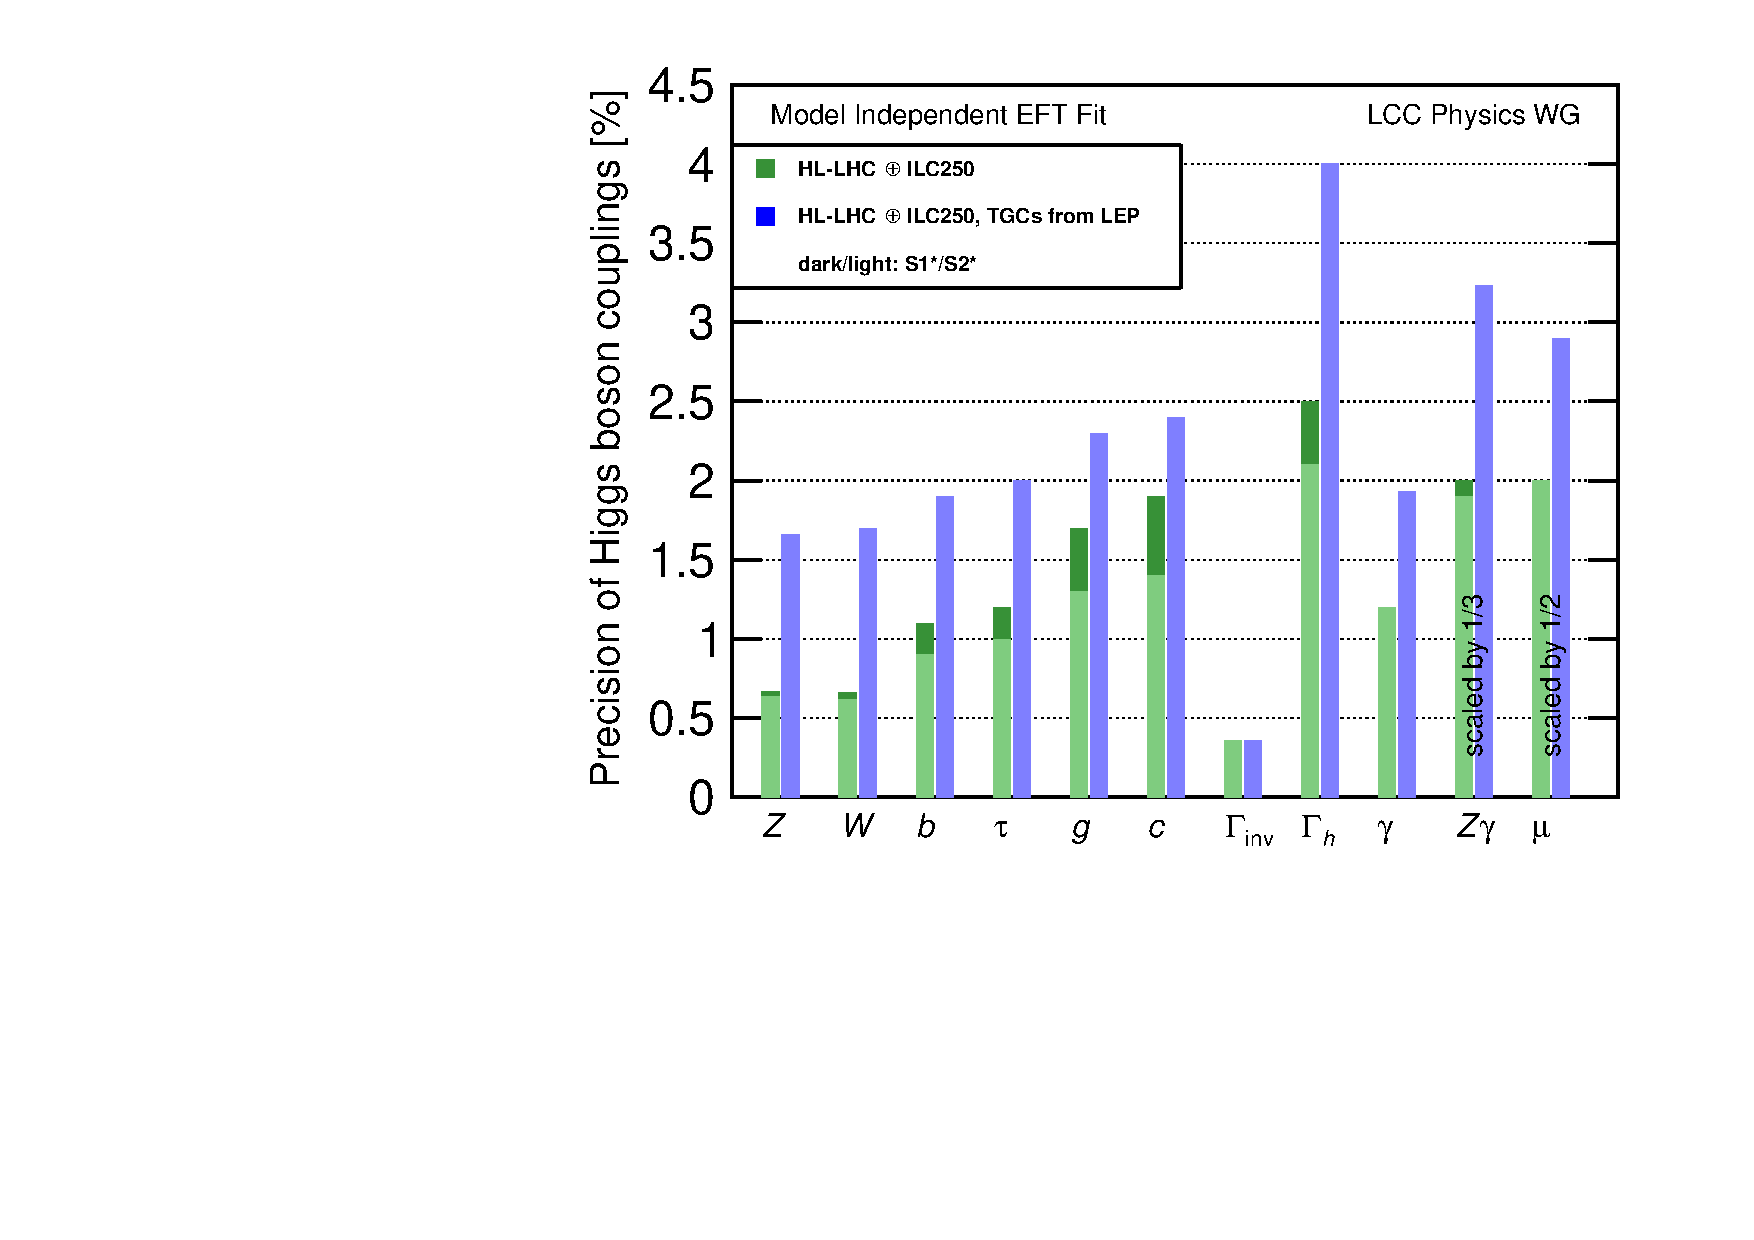
\includegraphics[width=0.7\hsize]{chapters/figures/DeltaHXX_SM_ILC_TGC_MI.pdf}
\caption{Projected Higgs boson coupling uncertainties assuming charged triple gauge coupling precisions as expected from ILC250 compared to using the corresponding LEP results instead. {\color{red}[Either here or in TGC section.]}}
\label{fig:oursimple}
\end{center}
\end{figure*}
%%%%%%%%%%%%%%%%%%%%%%%%%%%%%%%%%%%%%%%%%%%%%%%%%%%%%%%%%%%%%%



[discussion of the results]

%%%%%%%% to be moved to IX C %%%%%%%%%%%%%%%%%%%%%%%%%%%%%

{\color{red}[THE FOLLOWING IS TO BE MOVED TO
  SECTION~\ref{subsec:lincirc}; think about how this affects the
  linear/circular comparison]}\\
Figure~\ref{fig:polWIMPmanhattans} shows the 95\% CL reach in new physics scale $\Lambda$ for pair production of a light ($M_{X} = 1$\,GeV) WIMP mediated by a vector operator for different assumptions on luminosity, energy and polarization 
as they are typical for linear and circular colliders. In particular the polarised
configurations al refer to the ILC reference running scenario H20, see Sec.~\ref{sec:runscenarios}. Input to the limit calculation is the ILC study performed in full detector simulation of the ILD detector concept described in~Sec.~\ref{sec:searches}, and its extrapolation to other center-of-mass energies~\cite{Habermehl:417605}. The study includes a careful evaluation of the systematic uncertainties, comprising those on selection efficiencies, luminosity, beam energy (spectrum) and polarization as well as on the theoretical modelling of the background. The limit calculation uses a fractional event counting based on the 
energy spectrum of the photon. It can be seen that at 250\,GeV, 2\,\iab\ with polarized beams offer a greater reach than 5 or even 10\,\iab\ without beam polarization. Even at a higher center-of-mass energy of 350\,GeV, about 10\,\iab\ of unpolarised data  would be required to catch up with 2\,\iab\ of polarised data at 250\,GeV. The higher center-of-mass energies reachable by linear colliders, in conjuction with beam polarisation, improve the reach considerably. For instance the reach of the full H20 running scenario of the ILC roughly doubles the reach in $\Lambda$ compared to the 250\,GeV stage.

\begin{figure}
\centering
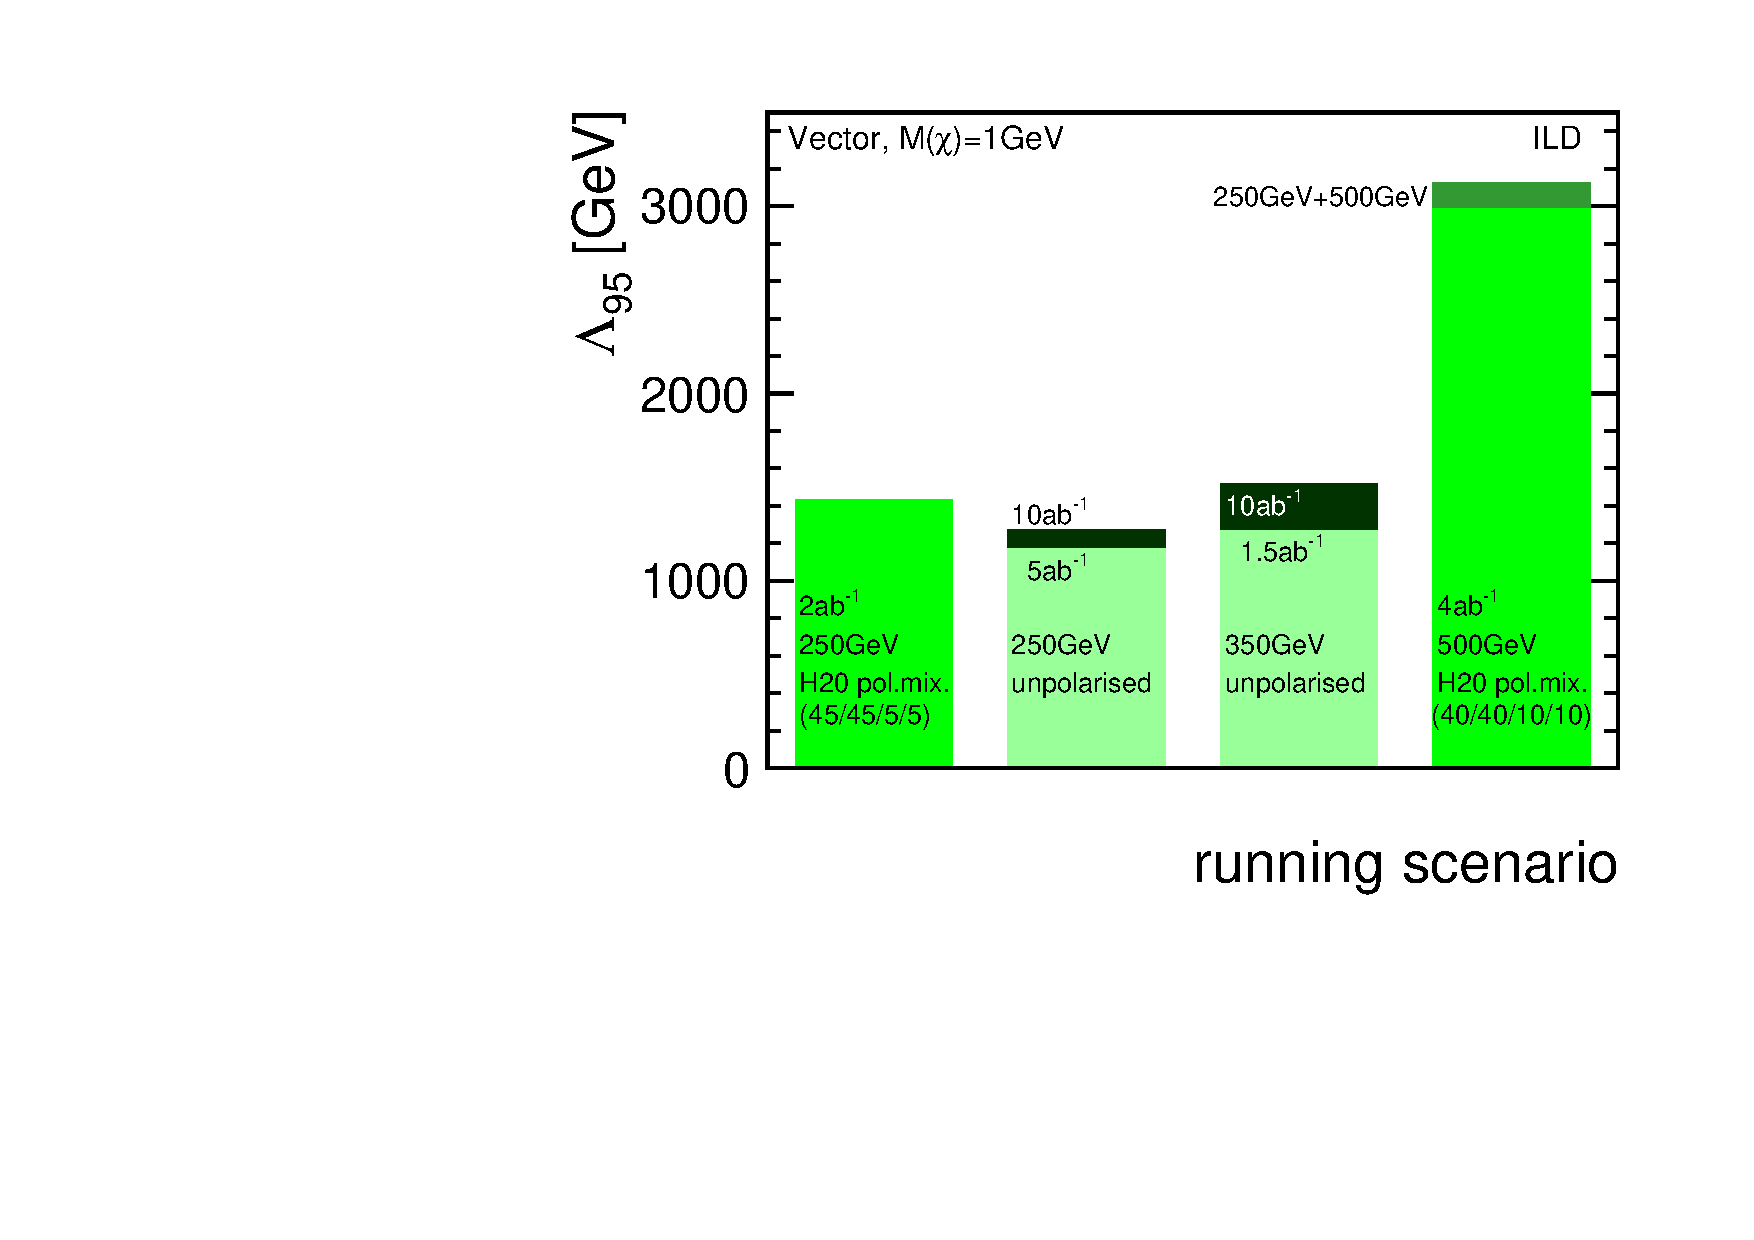
\includegraphics[width=0.95\linewidth]{./chapters/figures/manhattan_vector_v3.pdf}
		
\caption{{\color{red}[Michael, I think this plot and its description would better fit into section~\ref{subsec:lincirc}, but I didn't want to mess with `your' tex file. Please move it to your section if you like!]} Comparison of the reach for WIMP searches in the mono-photon channel for different assumptions on luminosity, polarization and energy, including systematic uncertainties (see Sec.~\ref{sec:searches} for a description of the analysis)~\cite{Habermehl:417605}. }
\label{fig:polWIMPmanhattans}
\end{figure}



\subsection{Comparison of the ILC and the HL-LHC Higgs capabilities}
\label{subsec:higgs:ilclhc}





Finally, we compare the capabilities of the ILC for precision Higgs
measurement to those of the HL-LHC.  Since the HL-LHC is approved,
while the ILC would be a new project, the ILC should be justified on
the basis that it will qualitatively advance our knowledge of the Higgs
boson over what is possible from the HL-LHC.  
This section will present several such comparisons.

The goal of the ILC is not simply to achieve a high degree of
precision in the measurement of Higgs boson couplings; it is to
discover deviations of the Higgs boson couplings from their Standard
Model predictions and to demonstrate those deviations with a high
degree of confidence.  The strengths of the ILC program are the
 following:
\begin{enumerate}
\item The ILC will report the properties of the Higgs boson in a
  highly model-independent framework.   Our estimate for the ILC capabilities
  are based on an effective field theory (EFT) model that includes
 {\underline{all}}\ dimension-6 operators that appear in the relevant physics
  cross sections at the tree level  (16 operators in all).   Our model
  also includes 2 further parameters to account for possible invisible
  and exotic Higgs decays.  The errors in this model due to
  unaccounted terms are percent-level corrections relative to the new
  physics effects already included in the model.   The analysis includes a
  high-precision determination of the Higgs boson total width. 
 Thus, the ILC will be able to measure  the full array of Higgs 
boson decays and to detect and quantify anomalies in any aspect of this behavior.
\item  For the Higgs boson couplings to $ZZ$, $WW$, and $b\bar b$, 
the ILC will achieve 1\% precision in its initial 250 GeV
  stage.   This is the
 level deemed necessary to be sensitive to the typical predictions 
of the effects of new physics models on the Higgs boson couplings.
\item  If  anomalies are  discovered in the ILC 
250 GeV program, these
  anomalies can be confirmed with an independent data set by
  increasing the energy of the ILC to 500 GeV.   This second energy
  stage will improve the precision of the ILC 
determinations by about a factor of 2.  
\item The ILC, with Higgs bosons tagged by recoil against a $Z$ boson
  and with no trigger requirements, will be able to observe directly
  all manner of exotic Higgs boson decays that might be produced by
Higgs couplings  to  light, weakly coupled  particles.
\end{enumerate}
All of these features go qualitatively beyond what is possible at the 
LHC, or at any hadron collider.

Beyond these conceptual improvements, we can compare the ILC
capabilities quantitatively to the projections released in the HL-LHC
Yellow Report \cite{YR}.   This comparison is given in
Table~\ref{tab:ILCLHC}.   It is not so straightforward to give a
direct apples-to-apples comparison to the estimates presented in the
Yellow Report.    The HL-LHC projections are reported in two
scenarios.  Scenario 1 (S1) is a projection based on our current
understanding of Higgs boson analyses, adding the increased data
available from the HL-LHC.   Scenario 2 (S2) assumes that the current
analyses can be improved by dividing the current theoretical
systematic errors by 2 and dividing the current experimental
systematic errors by $\sqrt{N}$, a factor of 6.   The latter
assumption, in particular, leads to very significant reductions in the
uncertainties.   S2 is intended to model the progress that the LHC
experiments have made in improving their understanding through actual
experience working with the data.  Still, ``past performance is not a 
guarantee of  future results''.

In spirit of the HL-LHC projections, we present multiple estimates of the ILC
capabilities at 250 GeV  in Table~\ref{tab:ILCLHC}.   We consider
these in turn.   The analysis labelled S1* in the table is based
on the highly model-independent framework described in item 1 above.
It is based on 2 ab$^{-1}$ of ILC data at 250~GeV on the reaction
$\ee\to hZ$.   To fix certain EFT operator coefficients, it also makes
use of data on $\ee \to W^+W^-$ at 250~GeV, as well as precision
electroweak measurements.   The analysis also includes
information from LHC that should be available from the 
HL-LHC results.  The LHC measurement of the ratio of the $\gamma\gamma$ and 
$ZZ^*$ branching ratios, which should be almost free of systematic
errors from the Higgs production process, plays an important role, and
the LHC measurments of the 
$\mu^+\mu^-$ and $Z\gamma$ branching ratios are used to constrain
those modes. 
The estimates of measurement errors
for the various ILC observables  are obtained as the result of  full
simulation studies using the ILD and SiD detector models.   The table
of input measurements is 
presented in some detail in Appendix A of \cite{Barklow:2017suo}. 

%%%%%%%%%%%%%%%
\begin{figure*}
\begin{center}
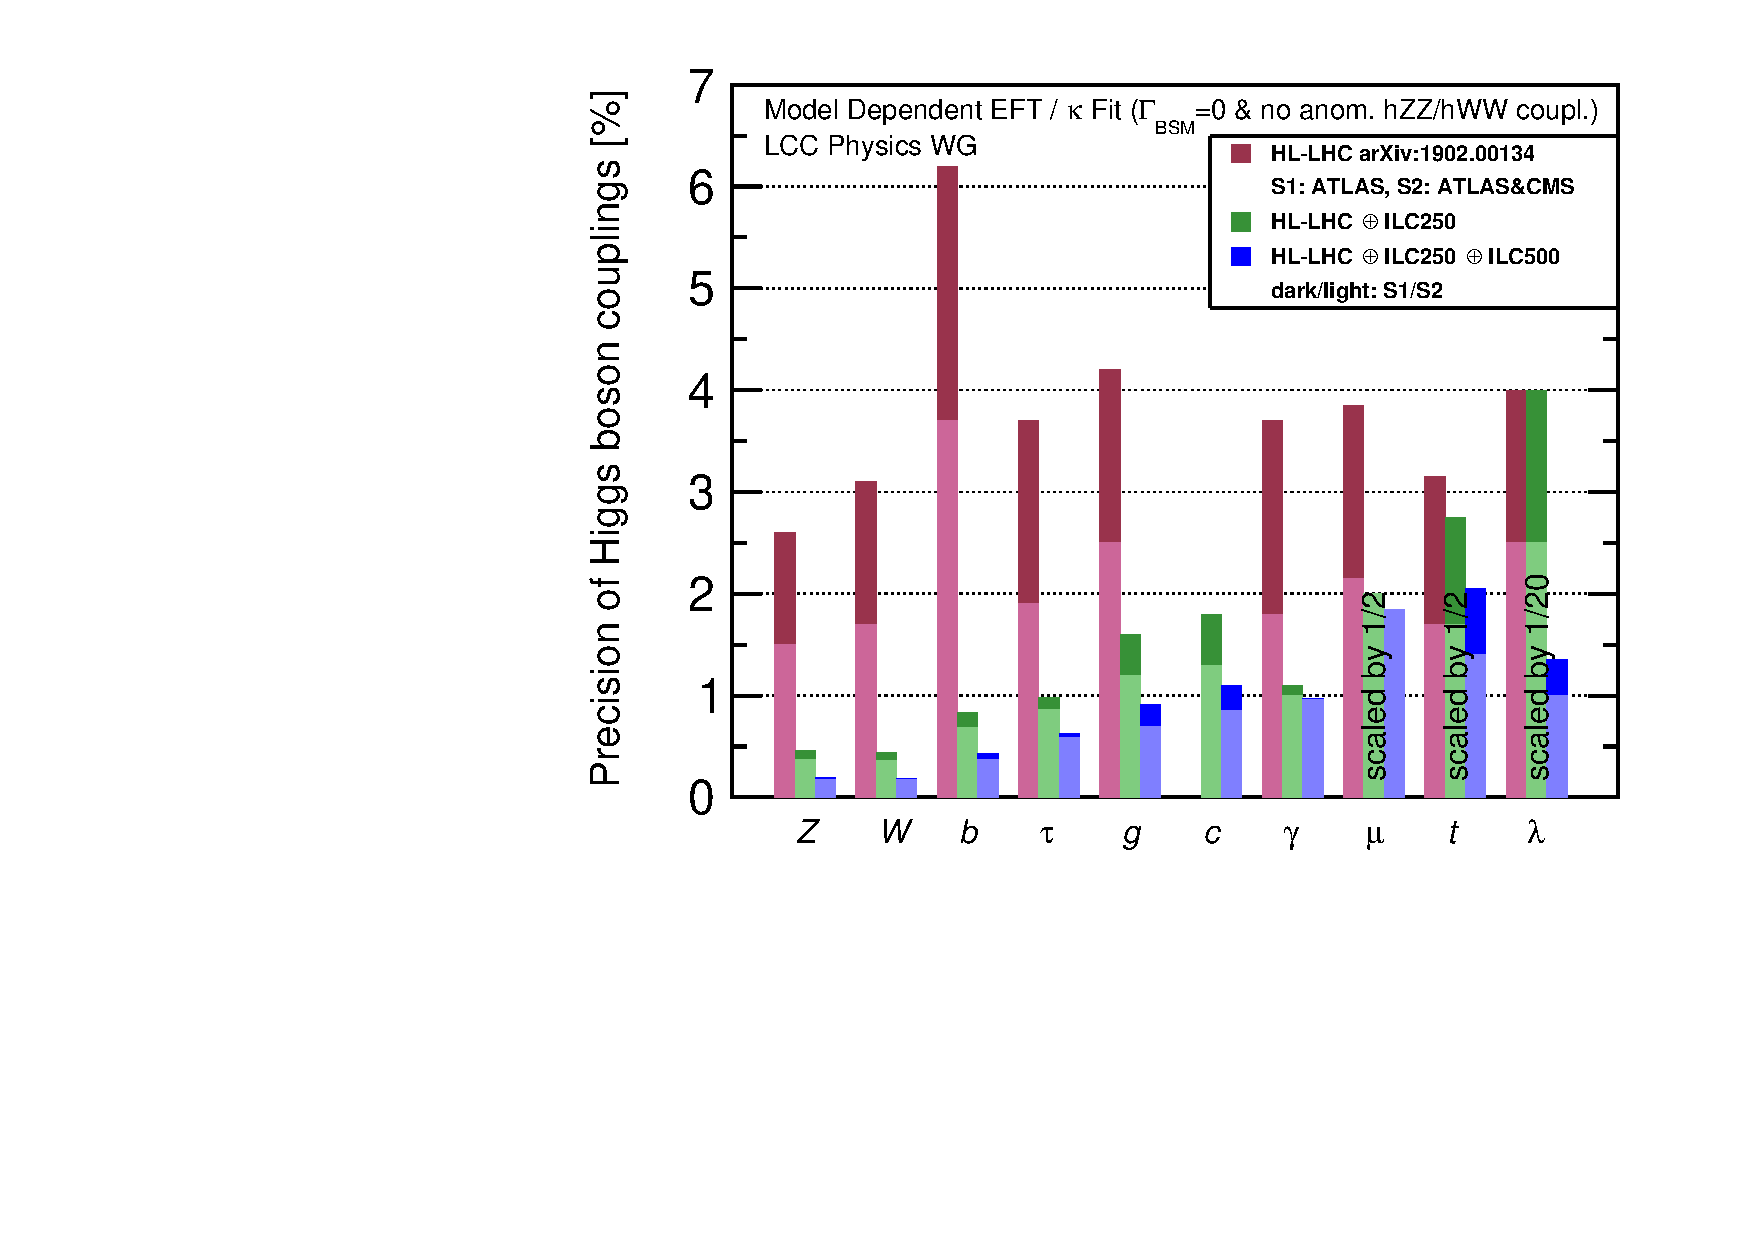
\includegraphics[width=0.7\hsize]{chapters/figures/DeltaHXX_SM_ILC_LHC_MD_S12.pdf}
\caption{Projected Higgs boson coupling uncertainties for the LHC and
  ILC
using the model-dependent assumptions appropriate to the LHC Higgs
coupling fit.   The
dark and light red bars represent the projections in the scenarios S1
and S2 presented in  \cite{YR}.    The dark and light green bars represent the
projections in the ILC scenarios S1 and S2 described in the
text.  The dark and light blue bars show the projections for scenarios S1 and S2
when
data from the 500~GeV run of the ILC is included.}
 \label{fig:ILCLHC}
\end{center}
\end{figure*}
%%%%%%%%%%%%%%%%%%%%%%%%%%%%%%%%%%%%%%%%%%%%%%%%%%%%%%%%%%%%%%


The LHC S1 estimates do not assume such a model-independent framework.
Among the many model-dependent assumptions in the LHC  analyses, two are
particularly important. They  assume  that the Higgs boson has no decay
modes beyond those predicted in the SM, and they  assume that the Higgs
boson couplings to $WW$ and $ZZ$ are modified only by a rescaling.  In
the ILC EFT analysis, each of these these couplings depends on two
independent constants, called $\eta_{W,Z}$ and $\zeta_{W,Z}$ in
\cite{Barklow:2017suo}.   We can redo the ILC EFT analysis
adding these two assumptions, that is, assuming no
Beyond-Standard-Model decays and assuming $\zeta_{W} = \zeta_Z = 0$.
This gives the uncertainty estimates listed for ILC  in the column S1
in Table~\ref{tab:ILCLHC}.   We consider the comparison of the S1
uncertainties the most direct comparison of the capabilities of  LHC
alone with results of adding the ILC dataset. 
  We emphasize that the S1 analysis is 
simply a recast of the S1* estimates; the ILC inputs are based just 
as firmly in our full-simulation results.

%%%%%%%%%%%%%%%%%%%%%%%%%%%%%%%%%%%%%%%%%%%%5
\begin{table}[!htbp]
\begin{center}
\begin{tabular}{lccccc}
   coupling     &  current  &    S1*     &     S1     &    S2*   &   S2   \\ \hline 
$HZZ$ - LHC  &     11.      &        &       2.4  &        &  1.5 \\ 
\phantom{$HZZ$} - ILC 250 &      &   0.67  &  0.46   &   0.64   &  0.37 \\ 
\phantom{$HZZ$} - ILC 500&      &   0.35  &  0.20  &  0.32   & 0.18 \\ 
 \hline 
$HWW$ - LHC  &    15.       &        &    2.6    &        &  1.7 \\ 
\phantom{$HWW$} - ILC 250 &      &   0.66 &  0.44   &   0.62  &  0.36 \\ 
 \phantom{$HWW$} - ILC 500 &      &   0.34 &  0.19   &  0.32 & 0.18 \\ 
   \hline 
$Hbb$ - LHC  &    29.       &        &         6.0   &        & 3.7 \\ 
\phantom{$Hbb$} - ILC 250 &      &  1.1  & 0.83   &   0.90   &  0.69 \\ 
\phantom{$Hbb$} - ILC 500 &      &  0.58  & 0.43   &  0.49  &  0.37 \\ 
 \hline 
$H\tau\tau$ - LHC  &    17.       &        &             2.8  &        & 2.8 \\ 
\phantom{$H\tau\tau$} - ILC 250 &      &  1.2  &  0.98   &   1.0  &  0.86 \\ 
\phantom{$H\tau\tau$} - ILC 500 &      &  0.75  &  0.63   &  0.67   & 0.59 \\ 
    \hline 
$Hgg$ - LHC  &     15.      &        &            4.0   &        &
               2.5  \\ 
\phantom{$hgg$} - ILC 250 &      &  1.7  &  1.6   &   1.3   &  1.2 \\ 
 \phantom{$hgg$} - ILC 500 &      &  0.95  &  0.91   &  0.74  & 0.70 \\ 
\hline 
$Hcc$ - LHC  &    -       &        &           -  &        &  - \\ 
\phantom{$Hcc$} - ILC 250 &      &   1.9  &  1.8   &   1.4  &  1.3 \\ 
\phantom{$Hcc$} - ILC 500 &      &  1.2  &  1.1   &   0.9  &  0.85 \\ 
    \hline 
$H\gamma\gamma$ - LHC  &    15.       &        &        2.9  &        & 2.8 \\ 
\phantom{$H\gamma\gamma$} - ILC 250  &      &   1.2  &  1.1  &   1.2   &  1.0\\ 
 \phantom{$H\gamma\gamma$} - ILC 500  &      &   1.0  &  0.97 &   1.0  &  0.96\\ 
\hline 
$H\mu\mu$ - LHC  &   70.        &        &    6.7  &        & 4.3 \\ 
\phantom{$H\mu\mu$} - ILC 250 &      &  4.0  &  4.0  &  4.0  &  4.0 \\ 
\phantom{$H\mu\mu$} - ILC 500 &      &  3.8  &  3.7  &  3.8  & 3.7\\ 
     \hline 
$Htt$ - LHC  &   14.        &        &           5.5   &        &  3.4
  \\  
 \phantom{$Htt$} - ILC 500  &        &    6.3    &     4.1     &    4.5   & 2.8
\\ 
\hline 
$HHH$ - LHC  &         &        &  80  &        &    50
  \\  
 \phantom{$HHH$} - ILC 500  &        &    27  &    27      &   20  & 20
\\ 
\hline \hline
$\Gamma_{tot}$ - ILC 250 &  &   2.5   &   1.4    &    2.1   & 1.1   \\ 
\phantom{$\Gamma_{tot}$} - ILC 500 & & 1.6 & 0.70 & 1.3  &  0.60  \\  \hline
$\Gamma_{inv}$ - ILC 250 &  &   0.36   &    -     &   0.36   &   -  \\ 
\phantom{$\Gamma_{inv}$} - ILC 500 & & 0.32 &  - & 0.32  & - \\  \hline
\end{tabular}
\end{center}
\caption{ \label{tab:ILCLHC}   Projected uncertainties in the Higgs
  boson couplings for LHC and for for ILC at 250~GeV, with the
  specific LHC input described in the text, 
in various scenarios.   All values
  are given in percent (\%). The values labeled ``current'' are taken
  from Table 8 of the CMS publication \cite{Sirunyan:2018koj}.   The
  LHC S1 values are those from the $\kappa$ fit to CMS projections,
  given in Tab.~36 of Ref.~\cite{Cepeda:2019klc}; the ATLAS projections are
  similar.    The S2 values are those from the ALTAS/CMS combination
  given in  Fig.~30 of Ref.~\cite{Cepeda:2019klc}.  Values for the HHH
  coupling are found in the text of Sec.~3.2 of 
Ref.~\cite{Cepeda:2019klc}. For ILC, the S1*
  results are those presented in Sec.~\ref{subsec:global:elements} for
  ILC programs at 250~GeV and 500~GeV.   The scenario S1 includes the 
same values for ILC measurement uncertainties but the  includes additional
model-dependent assumptions that are used in the LHC S1 analysis.
These are described in the text.  The
scenarios
S2* and S2 assume the improved performance in ILC measurements
presented in Sec.~\ref{subsec:higgs_improve}..  We believe that the 
comparison of the S1
  values  gives the sharpest comparison between the capabilities of LHC
  alone and the capabilities after adding the ILC measurements. }
\end{table}

We have also attempted to produce a set of S2 estimates for the ILC.
These, by construction, go beyond our current understanding.  But it
has been true for electron colliders, just as for hadron colliders,
that actual experience in operating the experiments and working with
the 
data has led  to results that have exceeded the design levels of
performance.  To estimate the possible improvement, 
we have looked for elements in our work that 
are conservatively estimated and for which more detailed effort
making use of actual experience could produce a substantial
improvement.  Most of the improvement factors that we incorporate here
have already been estimated in 
preliminary ILD and SiD analyses.   There is also 
headroom in the ILC design for a possible
increase in luminosity (for example, by improving the tolerances in
the damping rings), but this is not included in our estimates.
  Using the more 
optimistic values as inputs to our 
model-independent analysis, we find the
uncertainties in the column S2*.  Applying also the model-dependent
assumptions
 listed above, we find the uncertainties shown in
 the column S2. 


Figures~\ref{fig:ILCmodelindep} and \ref{fig:ILCLHC}  illustrate the
capabilities of the ILC and the comparison of the ILC and LHC
projections.  Figure~\ref{fig:ILCmodelindep} shows the uncertainty
projections for the 250~GeV stage of the ILC, in the highly
model-independent framework S1*.  In the figure, these results are
compared to results obtained in the same framework with the addition
of data from an energy upgrade to 500~GeV.   This justifies the
statement made above that deviations from the SM seen at the 250~GeV
stage of the ILC can be confirmed with an independent data set after
the upgrade to higher energy.   Figure~\ref{fig:ILCLHC} shows the
comparison of the ILC projections in the S1 and S2 scenarios to the 
projections given for the S1 and S2 HL-LHC scenarios given in
\cite{YR}.  
Note that, while the improvement from the S1 to S2 scenarios is a
matter of conjecture, the improvement from the 250~GeV to the 500~GeV
values is based on completed full-simulation studies.
